\documentclass[%
thesis=student,% bachlor's or master's thesis
coverpage=false,% do not print an extra cover page
titlepage=false,% do not print an extra title page
headmarks=true, % headmarks can be switched on or off
german,% or `english`
font=libertine, % use `libertine` font; alternatives: `helvet` / `palatino` / `times`
math=newpxtx, % math font `newpxtx`; alternatives: `ams`, `pxtx`
BCOR=5mm,% binding correction - adapt accordingly
coverBCOR=11mm% binding correction for the cover - adapt accordingly
]{tumbook}

\makeatletter %redefine some labels from the TUM template
\provideName{\@tum@examiner@}{Supervisor}{Themensteller} % or `Themenstellerin`
\provideName{\@tum@supervisor@}{Advisors}{Betreuer} % or `Advisor` / `Betreuerin`
\makeatother

\usepackage{booktabs}% for more beautiful tables
\usepackage{cleveref}% intelligent references

\usepackage{diffcoeff}
\usepackage{amsmath}
\usepackage{amsthm} % For theorem environments
\usepackage{mathtools}
\newtheorem{definition}{Definition}[section]
\newtheorem{lemma}{Lemma}
\newtheorem{theorem}{Theorem}

%Literatur
\usepackage[%
    backend=bibtex, %, or `biber` on more up-to-date systems
    sortcites, % sort automatically
    sorting=nty, % sort order
    safeinputenc, % solves problems with unicode-formatted author names etc.
    citestyle=alphabetic, %
    bibstyle=alphabetic, %
    hyperref=true, % provide clickable links
    maxbibnames=3, % shorten author list for more than 3 names
    maxcitenames=3, % use at most 3 names for key
    url=false, % do not print URLs
    doi=false, % do not print DOIs
    giveninits=true,
    ]%
{biblatex}
\addbibresource{literature.bib}

% automatische Anführungszeichen
\usepackage[autostyle=true]{csquotes}


\title{ROSA Method}
\subtitle{and its application}

\author{Jakob Dichgans}

\degree{Bachlor of Science}% or `Bachlor of Science`
\dateSubmitted{31. März 2023}% preferably use some universally recognized date format

\examiner{Prof.\@ Dr.\@ rer.\@ nat.\@ Adolf Hurwitz}% `Themensteller`
\supervisor{Dr.\@ L. Euler\\Dr.\@ C.-F. Gauß}% `Betreuer`


\begin{document}

\frontmatter
\maketitle

\section*{Zusammenfassung}
Eine kurze Zusammenfassung der Arbeit auf Deutsch.

\section*{Abstract}
A brief abstract of this thesis in English.

\cleardoublepage{}

\tableofcontents

\mainmatter{}
\chapter{Introduction}

\section{General Motivation for EWS}%
\label{sec:General Motivation for EWS}



We take the motivation for the ROSA method from \cite{Clarke:2023} and \cite{Scheffer:2009}.\\
Paleoclimate records suggest that critical thresholds of major components of the Earth system were crossed in the past \cite{Brovkin:2021}, where major parts of the Earth's system abruptly shifted from one state to another. Relatively small changes in the external forcing, such as a change in the greenhouse gas concentrations or incoming solar radiation can cause these rapid shifts. Since the raise of global temperatures, primarily due to burned fossil fuels, there is a growing concern \cite{Lenton:2019,Steffen:2018,Ritchie:2021} that key Earth System components (called "Tipping Elements") will cross Tipping points (TP) in the future and will undergo fast irreversible transitions \cite{Lenton:2008}. In some cases like the Greenland ice sheet there is concern, that a TP might already been crossed.
The crossing of a tipping point and transition to a qualitatively different state can be mathematically understood as a bifurcation. The critical thresholds are often crossed due to a small change in a parameter describing the forcing of the system. Although different types of bifurcation exist \cite{Ashwin:2012}, we will focus on bifurcation induced tipping (B-tipping) and especially fold bifurcations. Today different elements of the Earth system like the Atlantic Meridional Overturning Circulation (AMOC) \cite{Stommel:1961}, the Amazon Rain forest \cite{Cox:2000}, the permafrost \cite{Steffen:2018} or the Greenland ice sheet \cite{Feldmann:2015} are considered to be potential tipping elements. Several abprupt shifts were observed in the Coupled Model Intercomparison Project - Phase 5 \cite{Taylor:2012} and other earth system models (ESMs) \cite{Drijfhout:2015}, providing evidence that tipping points might occur. The crossing of tipping points would have  severe impacts and including tipping points in integrated assessment models (IAMs) would significantly increase the Social Cost of Carbon \cite{Dietz:2021}. Many people would face significant problems as studies of specific tipping point impacts have shown: an AMOC collaps would threat to halt large parts of arable farming in the UK \cite{Ritchie:2020} and there would be a higher risk of fires for communities in high altitudes due to the self-heating of soils \cite{Clarke:2021}.    \\
Knowing the exact thresholds for TP's would be useful but is out of reach \cite{Steffen:2018,Drijfhout:2015}. Nevertheless there are common characteristics for systems approaching a B-tipping, due to the theory of Normal Forms \cite{Strogatz:2015,Guckenheimer:1983}. The most important one is \emph{critical slowing down} (CSD). In genereal systems return back to equilibrium after a small perturbation. As the system approaches a tipping point this return-time increases \cite{Scheffer:2012}, the variance will increase and its autocorrelation tends to unity \cite{Scheffer:2009,Held:2004}. The latter two statistical indicators are considered traditional 'Early Warning Signals' (EWS). (Care with EWS ?). We will discuss CSD and the theory behind these EWS more in detail in the following chapters. \\
The traditional early warning signals were applied to paleoclimate data and detected TP's \cite{Boers:2018}. They were applied to a 5-year resolution time series obtained from the raw North Greenland Ice Core Project (NGRIP) record to indicate the arrival of the Dansgaard–Oeschger (DO) events. These EWS also suggest the approach of TP's in the Greenland Ice Sheet \cite{Boers:2021} and in the AMOC  \cite{Boers:2021b} following the rise of global temperatures. Despite the succesful applications of the tradtitional EWS they also have a flaw. They depend on a stationarity assumption of the process, something which is often violated in nature, yielding the risk of false positiv or false negative signals. We will give examples for this later. 

Although we are interested here mainly in climate science as an application, the theory of EWS for TP's can be applied in many other contexts of complex dynamical systems as well. Systemic failures like asthma attacks \cite{Venegas:2005} or epileptic seizures in medicine \cite{Litt:2001, McSharry:2003}, market crashes in finance \cite{Kambhu:2007,May:2008} or catastrophic shifts in wildlife or fish populations for ecosystem services \cite{Scheffer:2001, MillenniumEcosystemAssessment:2005}. 

In figure \ref{fig:1.1} we show different ways of how the equilibrium state of a system can react to changes in the conditions of the system. In the four panels we plot the equilibria states as a function of a bifurcation parameter representing the conditions of the system. The solid black lines illustrate stable states and the dashed black lines in panels c and d illustrate unstable ones. Additional grey arrows indicate the direction of movement of the system if it is outside of equilibrium. If the system is close to a tipping point like F2 a small change in the conditions (Panel c) or a small perturbation (Panel d) can lead to a sudden large shift in the system state. Panel b gives an example for a scenario where in the absence of a real bifurcation a small change in a critical area of the conditions can still lead to a large shift of the state. In Panel a the large change in the system state is caused by a large external forcing. We will focus on the fold bifurcation scenarios of c and d for testing purposes of the EWS and give an example of a simple climate model in the end where such a bifurcation also arises.


% In the Earth system the noise corresponds to external drivers of the system, which are not included in the model. Often this key assumption is violated, eg. due to oscillatory variability in the Earth System (C:28). An example is the El-Nino Southern Oscillations which has a large impact on the Amazon Rainforest - a potential tipping element (C:29). (Incompatability with long memory process (30,31) ?). Relaxing the assumptions on the noise can change the characteristics of the traditional EWS or can make them disappear (C:31). Hence EWS without an assumption on the noise would be of use. 


\begin{figure}[t]
    \centering
    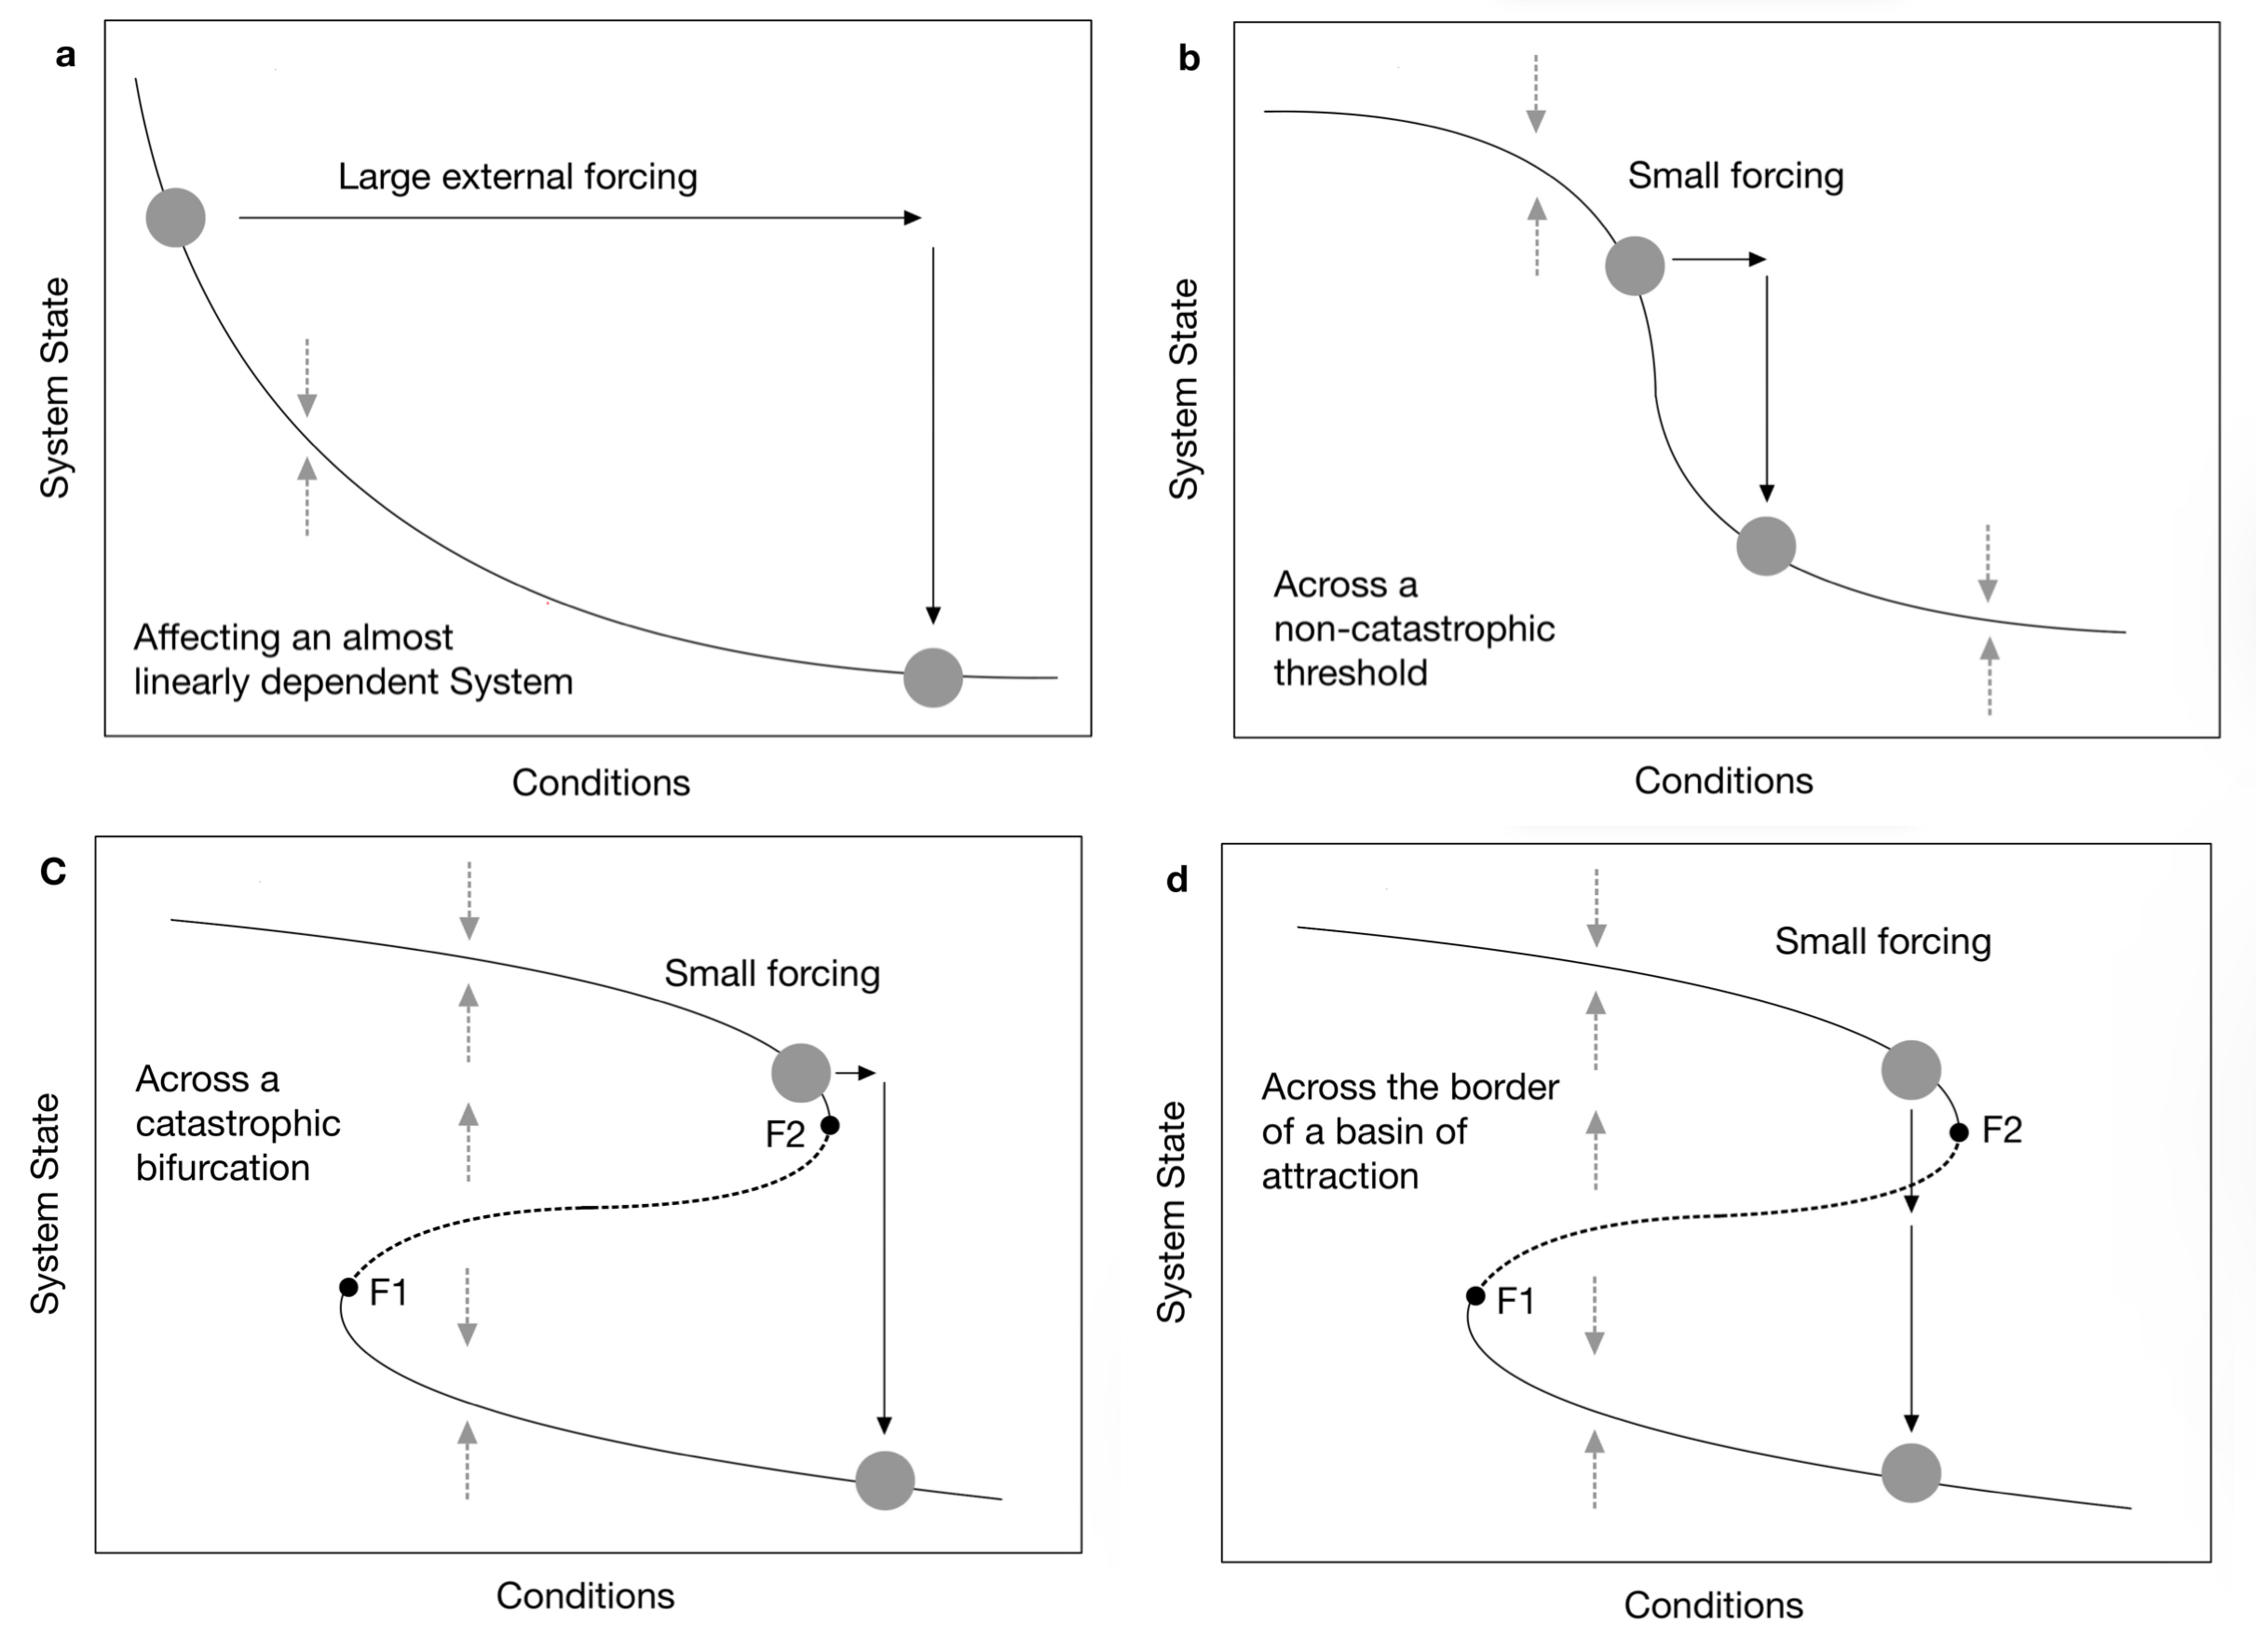
\includegraphics[width=0.8\textwidth]{bachelor-thesis/figures/scheffer_box_1.jpg}
    \caption{Critical transitions in the fold catastrophe model, modified from \cite{Scheffer:2009} Box 1}
    \label{fig:1.1}
\end{figure}


\section{Motivation for the traditional EWS: Variance and $AC(1)$}
\label{sec: Motivation for the traditional EWS: Variance and $AC(1)$}

We take this section mainly from \cite{Scheffer:2009}.\\
The goal of early warning signals is to indicate the approaching of a tipping point in our system. Most indicators make use of the CSD phenomenon, which we want to illustrate with a simple example. The main idea behind CSD is the following: Assume we have a stochastically forced dynamical system of the form 
\begin{equation}
    \frac{dx}{dt} = f(x(t),\mu(t)) + \xi (t) 
    \label{stochastically forced system}
\end{equation}

where $\mu(t)$ is a bifurcation parameter and $\xi(t)$ is a noise term following some probability distribution for every $t \geq 0$. The system has a fold bifurcation point at $\mu_{c}$. 
We can linearize around an equilibrium $x^{*}$:
        \[
        f(x;\mu) \approx f(x^{*}(\mu),\mu) + \partial_{x}f(x^{*}(\mu);\mu)(x(t)-x^{*}) = \partial_{x}f(x^{*}(\mu);\mu)(x(t)-x^{*}) =: -\lambda(\mu)(x(t) - x^{*})
        \]
        
To improve legibility we omitted the time dependence of the bifurcation parameter. Now CSD gives us that for $\mu \rightarrow \mu_{c}$ we can expect that the linearized restoring rate $\lambda(\mu)$ will go to zero. Hence the system will be slower in recovering from perturbations when it approaches the TP at $\mu_{c}$. This phenomenon occurs for all continous models approaching a fold bifurcation \cite{Wissel:1984}. Furthermore CSD was observed in several models already far away from the bifurcation point \cite{VanNes:2007}. Now we give a simple example to illustrate the relationship between the recovery rate $\lambda(\mu)$ and proximity to a TP, following \cite{Scheffer:2009} Box 2. To do so, we consider the following system: 
\begin{equation}
    \frac{dx}{dt} = \gamma (x-a)(x-b) =: f(x) \label{eq:1}
\end{equation}
with $a,b,\gamma \in \mathbb{R}$, $a < b$ and $\gamma > 0$. The two stationary states of the system are $a$ and $b$, where $a$ is stable and $b$ is unstable. Assume $b$ is fixed and $a$ is the bifurcation parameter.
We have: 
\[\lambda (a) = -\frac{df}{dx}|_{a} = \gamma(b-a)\] 

We will now study how the system evolves if we add a small perturbation to the stable state a. Let $\epsilon(t) := x(t) - a$. We have:

\[
\frac{d\epsilon(t)}{dt} = \frac{d(a + \epsilon(t))}{dt} = f(a + \epsilon(t)) \approx 
 -\lambda(a)\epsilon(t)
\]
The solution is $\epsilon(t) = \epsilon_{0}exp(-\lambda(a)t) = \epsilon_{0}exp(-t/T_{R}(a))$, where $T_{R}(a) := 1/ \lambda(a)$ is the characteristic return time \cite{Wissel:1984}.
We see that for $a \nearrow b$ it holds that $\lambda(a) \searrow 0$ and $T_{R}(a)\nearrow \infty$. In this case the restoring rate $\lambda(a)$ is linearly dependent on the size of the basin of attraction.

From CSD we know that the recovery rate after a small disturbance of a system is an indicator for proximity to a bifurcation point \cite{VanNes:2007}. In natural systems it is mostly not possible to test recovery rates directly. Still, since most systems are under constant natural perturbation we can use statistics and try to deduce information about the linear restoring rate. An increase in the autocorrelation of a time series generated by equation \ref{stochastically forced system} is one important predictor for slowing down \cite{Ives:1995}. This is easy to understand intuitively: Due to the decrease in recovery rate of the system the states get more and more similar to each other. The lag-1 autocorrelation measures how closely the current state is correlated to the past state. Hence we expect an increase in this measure.

Another indicator for an approaching TP is an increase in the variance of the fluctuations of a stochastically forced system. The intuitive explanation is again simple: When the linear restoring rate goes to zero, the reverting back to the equilibrium gets very slow and the perturbations can accumulate leading to the increase in the variance. 
We will prove these properties of the traditional EWS later more formally. To do so we first introduce some concepts in the following chapter Prerequisites. In Figure \ref{fig:scheffer_fig_1_reimp} we give more intuition for the traditional EWS methods. \\



\begin{figure}[h]
    \centering
    \includegraphics[width=0.8\textwidth]{reimp_scheff_fig_1.jpg}
    \caption{Modified from \cite{Scheffer:2009}, Figure 1:
    Two time series are simulated by the SDE: $dX_{t}=X(1-X/K)-c(X^2/(X^2+1))dt + dW_{t}$ modelling a harvested population with carrying capacity $K = 10$ and maximum harvest rate c (0.5 for high resilience and 2.3 for low resilience). In Panels a,b,c the system is farther away from the TP: the restoring rate is higher and the basin of attraction is smaller. This leads to a smaller variance in the fluctuations around the equilibrium and a smaller autocorrelation. Panels d,e,f show the system being closer to the TP: the restoring rate is lower and the basin of attraction is larger. There is a larger variance and autocorrelation.}
    \label{fig:scheffer_fig_1_reimp}
\end{figure}



\chapter{Prerequisites}


\section{Probability theory \& Statistics}

We start with some definitions, which we will need later.

\begin{definition}[Stochastic process (PT script definition 5.1)]
Let I $\subseteq \mathbb{R}$. Let $X_{t}:\Omega \rightarrow \mathbb{R}, t \in I$ be a random variable on the same probability space $(\Omega,\mathcal{F},P)$. Then, $X = (X_{t})_{t \in I} $ is called a real-valued stochastic/random process. If $I = \mathbb{N}_{0}$ it is a discrete time process, if  $I = \mathbb{R}_{+}$ it is a continuous process.
\end{definition}


\begin{definition}[Gaussian process]
    A stochastic process $(X_{t})_{t\geq 0}$ is a Gaussian process if for all $t_{1} < t_{2} < ... < t_{n}$, the vector $(X_{t_{1}},...,X_{t_{n}})$ is a Gaussian process.
\end{definition}


\begin{definition}[Autocovariance function]
Be $(X_{t})_{t \in I \subseteq \mathbb{R}}$ a random process. We define the autocovariance function: 
\[
R_{X}(t_{1},t_{2}) := Cov(X_{t_{1}},X_{t_{2}})
\]    
\end{definition}

It is called 'auto'-covariance function, because the covariance is taken with respect to the same process $X_{t}$


%stanf_stat_proc
\begin{definition}[weak sense stationarity]
A stochastic process $(X_{t})_{t\geq 0})$ is weak-sense stationary (WSS), if:

\begin{subequations}
    \begin{align}
        E[X(t)] &= \mu \ \ \forall t \geq 0 \\
        R_{X}(t_{1},t_{1} + \tau) &= R_{X}(t_{2},t_{2} + \tau) \ \ \forall t_{1},t_{2},\tau \in \mathbb{R}_{+} \\
        E[X(t)^2]&<\infty
    \end{align}
\end{subequations}   
\end{definition}

Since $R_{X}(t_{1},t_{2}) = R_{X}(t_{2},t_{1})$, $R_{X}$ is a function of $\lvert t_{2} - t_{1} \rvert$ for a WSS stochastic process and can be written as:
\[
R_{X}(\tau) := R_{X}(t,t + \tau), \ \tau \geq 0
\]

As the name suggests there is also a stronger concept of stationarity called \textit{Strong Sense Stationarity} (SSS). The latter always implies WSS, while the reverse direction isn't true in general. However it holds for gaussian processes (?). We will only need WSS.

Now we can also define the autocorrelation function for WSS-processes:

\[
\text{AC}(\tau) := \frac{R_{X}(\tau)}{(\text{Var}(X_{t})\text{Var}(X_{t+\tau}))^{\frac{1}{2}}}, \ \tau \geq 0
\]


\begin{definition}[AC]
Let $(X_{t}) = (X_{0},...,X_{n}) \in \mathbb{R}^{n+1}$ be a time series with mean $\Bar{X}$. The $\widehat{AC(1)}$ or lag-1-Autocorrelation is defined by: 
\[
\widehat{AC(1)} = \frac{\sum_{t=0}^{n-1}(X_{t}-\Bar{X})(X_{t+1}-\Bar{X})}{\sum_{t=0}^{n}(X_{t}-\Bar{X})^2}
\]
\end{definition}

The following Lemma gives a connection between the AC(1) and the linearized restoring rate (\cite{Morr:2024} SM2): 

\begin{lemma}
    Let $(X_{t})_{t\geq 0}$ be a centered gaussian process. Then it holds for all $\epsilon > 0$:
    \[
    E[\frac{X_{k+1}-X_{k}}{X_{k}}1_{\{\lvert X_{k} \rvert > \epsilon\}}] = AC(1) - 1
    \]
\end{lemma} 

Later we want to compare our EWS indicators. Then we need to quantify how monotone increasing a series of values is. For this we will use the kendall tau coefficient. 

\begin{definition}[Kendall's $\tau$ coefficient]
\label{def:Kendall tau}
Let $(x_{1},y_{1}),(x_{2},y_{2}),...,(x_{n},y_{n})\in \mathbb{R}^{2}$. A pair of observations $(x_{i},y_{j}),(x_{j},y_{j}), i,j \in [n]$ is concordant if it holds:
\[
((x_{i} > x_{j}) \wedge (y_{i} > y_{j})) \vee
((x_{i} < x_{j}) \wedge (y_{i} < y_{j}))
\]
Otherwise it is discordant. The Kendall $\tau$ coefficient is defined as:
\[
\tau := \frac{\#concordant\ pairs - \#number\ of\ discordant\ pairs}{\#pairs} = \frac{2}{n(n-1)}\sum_{i<j}sgn(x_{i}-x_{j})sgn(y_{i}-y_{j})
\]
where sgn is the signum function    
\end{definition}


\section{Stochastic analysis}

\begin{definition}[Wiener process (SA script Def. 1.6)]
A Wiener process is a stochastic process $(W_{t})_{t\geq 0}$ on some probability space $(\Omega,\mathcal{F},P)$ with the following properties: 
\begin{itemize}
    \item $W_{0} = 0$ P-a.s
    \item For $0 = t_{0} < t_{1} < ... < t_{n}$, the increments $W_{t_{i}} - W_{t_{i-1}}, 1 \leq i \leq n$, are independent with law $N(0,t_{i}-t_{i-1})$
    \item $t \mapsto W_{t}(\omega)$ is continuous for P-a.a $\omega \in \Omega$
\end{itemize}
\end{definition}

Interpretation: 

\begin{itemize}
    \item $t \mapsto W_{t}(\omega)$ is one random evolution in time
    \item $(W_{t})_{t \geq 0} : \Omega \mapsto C[0,1]$ is a random variable that takes an $\omega$ as input and outputs one realization of a path
\end{itemize}

We define the \textit{Cameron-Martin-Space} as:
\[
H_{t} := \{ h \in C[0,t]: \exists f \in L^{2}[0,t] \ s.t \  h(s) = \int_{0}^{s} f(\tau) d\tau, 0 \leq s \leq t \}
\]

For $h \in H_{t},\ f \in L^{2}[0,t]$ is uniquely determined and we write: 
\[
h' = f
\]
(In genereal $h$ does not have to be differentiable for every $s \in [0,t]$)

Now we can define stochastic integrals for a certain class of functions:

\begin{lemma}[The Paley-Wiener stochastic integral (SA script Lemma 3.4)] 
Let $(W_{s})_{s\geq 0}$ be a Wiener process and $h \in H_{t}, t \geq 0$. Then:
\[
\xi_{n}^{t} := 2^{n}\sum_{j=1}^{2^{n}}(h(\frac{tj}{2^{n}})-h(\frac{t(j-1)}{2^{n}}))(W_{\frac{tj}{2^{n}}}-W_{\frac{t(j-1)}{2^{n}}}) 
\]

converges P-a.s and in $L^{2}$. We denote the limit by
\[
\int_{0}^{t}h'(s)dW_{s} = \int_{0}^{t}h'dW
\]
\end{lemma}

At this point we want to highlight the importance in the definition of the Wiener process that the variance of $W_{t}$ is proportionate to time. Per definition it holds $W_{t} \sim N(0,t)$. Suppose another power $t^{\alpha}, \alpha > 0$ was chosen. 

It holds: $\int_{0}^{t} 1 dW_{s} = W_{t}$ and $Var[W_{t}] = t^{\alpha}$ by assumption. But: 
$Var[\xi_{n}^{t}] = Var\left[\sum_{j=1}^{2^{n}}\left(W_{\frac{tj}{2^{n}}} - W_{\frac{t(j-1)}{2^{n}}}\right)\right] = 2^{n}Var\left[W_{\frac{t}{2^n}}\right] = 2^{n}\left(\frac{t}{2^{n}}\right)^{\alpha}$, where we use that the increments are i.i.d. Since  $Var[\xi_{n}^{t}] \xrightarrow{n \rightarrow \infty} Var[W_{t}]$ (by the dominated convergence theorem (?)), $\alpha$ has to equal 1. \\

Consider the process:

\begin{definition}[Ornstein-Uhlenbeck process (SA script Example 10.7)] 
For $\alpha > 0$, $(W_{t})_{t\geq 0}$ a Wiener process, $x_{0} \in \mathbb{R}$. Consider the following SDE:
\[
dX_{t}^{(w)} = -\lambda X_{t}^{(w)} dt + \sigma dW_{t}, X_{0}^{(w)} = x_{0}
\]
or equivalently
\[
X_{t}^{(w)} = x_{0} - \lambda\int_{0}^{t}X_{s}^{(w)}ds + \sigma W_{t}, t \geq 0
\]  
\end{definition}

$\textbf{Claim}$: 
\[
X_{t} = \exp(-\lambda t)x_{0} + \sigma\int_{0}^{t}\exp(-\lambda (t-s))dW_{s}
\]
solves the above SDE. We check this applying Ito's product rule to $\sigma e^{-\lambda t}\int_{0}^{t}e^{\lambda s}dB_{s}$:
\[
dX_{t} = -\lambda x_{0}e^{-\lambda t}dt - \lambda\sigma(e^{-\lambda t}\int_{0}^{t}e^{\lambda s}dW_{s})dt + \sigma e^{-\lambda t}e^{\lambda t}dW_{t} = -\lambda X_{t} dt + \sigma dW_{t}
\]

If we choose $X_{0} \sim N(0,\frac{1}{2\lambda})$ as an initial distribution, which is independent of $(W_{t})_{t\geq 0}$ than $E[X_{t}] = 0$, $Cov[X_{s},X_{t}] = \frac{1}{2\lambda}e^{(-\lambda\lvert t-s \rvert)}$ for $t,s \geq 0$ and $X_{t}$ is wide sense stationary. It follows that $Var[X_{t}]=E[(X_{t})^{2}]=\frac{1}{2\lambda}$ and $X_{t} \sim N(0,\frac{1}{2\lambda}), \forall t \geq 0$, because the sum of normal random variables is again a normal random variable.

To proof the statements about the expectation and the covariance of $X_{t}$ we use some  results from stochastic analysis and probability theory.
From stochastic analysis we use a weeker form of Ito's isometry:

\begin{lemma}[Ito's isometry]
 Let $t \geq 0$ and $g \in L^2[0,t]$. Then:
 \[
 E[(\int_{0}^{t}g(s)dW_{s})^{2}] = \int_{0}^{t}g(s)^2ds
 \]
\end{lemma}

The following Lemma shows that $\int_{0}^{t}e^{\alpha s}dW_{s}$ is a martingale.   \textit{(I)}

\begin{lemma}
    Let $g \in L^2[0,t]$ for every $t \geq 0$. Then $(\int_{0}^{t}g(s)dW_{s})_{t\geq 0}$ is a martingale and hence:
    \[
    E[\int_{0}^{t}g(s)dB_{s}] = 0, \ \forall t \geq 0
    \]
\end{lemma}

From probability theory we use the following two results about conditional expectations:

\begin{lemma}
    Let $X: \Omega \rightarrow \mathbb{R}$ be an $(\mathcal{F}_{0},\mathcal{B}(\mathbb{R}))$- measurable random variable with $E[\lvert X \rvert] < \infty$ or $X \geq 0$ and $\mathcal{F} \subseteq \mathcal{F}_{0}$ a $\sigma$-algebra. Then it holds:
    \[
    E[E[X|\mathcal{F}]] = E[X]
    \]
\end{lemma}

\begin{lemma}
    If X is $\mathcal{F}$-measurable, $E[\lvert XY \rvert] < \infty$ and $E[\lvert Y \rvert]< \infty$ then:
    \[
    E[XY|\mathcal{F}] = XE[Y|\mathcal{F}], \ P-a.s
    \]
\end{lemma}

Let $0 \leq s \leq t$. Then:

\[
E[X_{t}] = e^{-\lambda t}E[X_{0}] + e^{-\lambda t}E[\int_{0}^{t} e^{\lambda s} dW_{s}] = e^{-\lambda t}E[\int_{0}^{t} e^{\lambda s} dW_{s}] \stackrel{(I)}{=}  0
\]

Next we want to prove: $Cov[X_{s},X_{t}] = \frac{1}{2\lambda}e^{-\lambda \lvert t-s \rvert}$. 
\begin{equation}
    Cov[X_{s}X_{t}]=E[X_{s}X_{t}] = e^{-\lambda(t+s)}E[X_{0}^{2}] + e^{-\lambda(t+s)}E[\int_{0}^{t}e^{\lambda u}dW_{u}\int_{0}^{s}e^{\lambda v}dW_{v}]
    \label{cov white noise noise}
\end{equation}

We show that for any martingale $(M_{t})_{t \geq 0}$ the following holds: 
\begin{equation}
    E[M_{t}M_{s}] = E[M_{s}^{2}], \ s \leq t
    \label{result cond exp}
\end{equation}

Lemma 5 gives us:
\[
E[M_{t}M_{s}] = E[E[M_{t}M_{s}|\mathcal{F}_{s}]]
\]
Since $M_{s}$ is $\mathcal{F}_{s}$-measurable, Lemma 6 yields:
\[
E[E[M_{t}M_{s}|\mathcal{F}_{s}]] = E[M_{s}E[M_{t}|\mathcal{F}_{s}]]
\]
For a martingale it holds: $E[M_{t}|\mathcal{F}_{s}] = M_{s}, s \leq t$. Equation \ref{result cond exp} follows. Continue with \ref{cov white noise noise}:


\begin{subequations}
    \begin{align*}
        E[X_{s}X_{t}] &= \frac{1}{2\lambda}e^{-\lambda(t+s)} + e^{-\lambda(t+s)}E[(\int_{0}^{s}e^{\lambda v}dW_{v})^{2}]   \\
         &= \frac{1}{2\lambda}e^{-\lambda(t+s)} + e^{-\lambda(t+s)}\int_{0}^{s}e^{2\lambda v}dv, \ \ \ (Lemma \ 3) \\
         &= \frac{1}{2\lambda}e^{-\lambda(t+s)} + e^{-\lambda(t+s)}\frac{1}{2\lambda}(e^{2\lambda s} - 1) \\
         &= \frac{1}{2\lambda}e^{-\lambda(t-s)} 
    \end{align*}
\end{subequations}   

\qed

Hence it holds for $\tau > 0$:
\[
R_{X}(\tau) =  \frac{1}{2\lambda}\exp(-\lambda\tau)
\]





\subsection{red noise in ct stoch modelling}
From \cite{Morr:2022}.

dynamical modelling usually consists of a deterministic part with an added noise term to capture the unresolved dynamics. Simple discrete time example:

\begin{equation}
    X_{k+1}-X_{k} = f(X_{k},k) + \sigma\epsilon_{k}, X_{0} = x_{0} \in \mathbb{R}
\end{equation}


an usual choice would be independent $\epsilon_{k} \sim \mathcal{N}(0,1)$, also called white noise. (why white noise noise?)[1].
However in some applications the assumption of independence may be unsuitable due to "persistence in time" of the unresolved dynamics [2,3].

One common way to model correlated noise is via an AR(1)-process:
\[
\epsilon_{k+1} = \phi\epsilon_{k} + z_{k}, \epsilon_{0} \sim \mathcal{N}(0,(1-\phi^2)^{-1})
\]
with $0<\phi<1$ and $(z_{k})_{k}\in\mathbb{N}$ iid standard Normal random variables. This type of noise is also called \textit{red noise}. Why red noise? With the specific choice of the distribution of $\epsilon_{0}$ the process is weakly stationary. We proof this only considering $\tau = 1$ for the autocorrelation function, since later we are only interested in $R_{X}(1)$. First we show, that: $\epsilon_{k} \sim \mathcal{N}(0,(1-\phi^2)^{-1}), \forall k \in \mathbb{R}$ by induction. Inductionstart: the statement holds for $\epsilon_{0}$ by definition.
Inductionstep: Suppose the statement holds for $k \in \mathcal{N}$. Then:

\begin{subequations}
    \begin{align}
        E[\epsilon_{k+1}] &= \phi E[\epsilon_{k}] + E[z_{k}]  = 0 \\
        Var[\epsilon_{k+1}] &= \phi^2 Var[\epsilon_{k}] + 1 = \frac{\phi^2}{1-\phi^2} + 1 = \frac{1}{1-\phi^2}     
    \end{align}
\end{subequations}   

by linearity of the expectation, properties of the variance, the induction hypothesis and the fact that $z_{k} \sim \mathcal{N}(0,1) \forall k \in \mathbb{N}$. Now to show that $R_{\epsilon}(k,k+1) = R_{\epsilon}(0,1) \forall k \in \mathbb{N}_{0}$ it suffices to show that $Cov[\epsilon_{k},\epsilon_{k+1}] = E[\epsilon_{k}\epsilon_{k+1}] - E[\epsilon_{k}]E[\epsilon_{k+1}] = E[\epsilon_{k}\epsilon_{k+1}] = E[\epsilon_{0}\epsilon_{1}] \forall k \in \mathbb{N}_{0}$. This follows from: 
\[
E[\epsilon_{k}\epsilon_{k+1}] = E[\epsilon_{k}(\phi\epsilon_{k} + z_{k})] = \phi E[\epsilon_{k}^2]
\]
and the fact that $\epsilon_{k}$ and $z_{k}$ are independent and that the $\epsilon_{k}$'s are identically distributed. ?how to prove general case?

The discrete time noise process has a exponentially decaying correlation structure $\epsilon_{k}$. Claim:
\[
R_{\epsilon}(\tau) = \frac{\phi^{\tau}}{1-\phi^{2}}, \tau \in \mathbb{N}
\]
Proof: \\
It holds: 
\[
R_{\epsilon}(0)= Var(\epsilon_{k}) = \frac{1}{1-\phi^{2}}
\]
Further it holds for $\tau \in \mathbb{N}_{0}$:
\[
R_{\epsilon}(\tau+1) = Cov[\epsilon_{k},\epsilon_{k+\tau + 1}] = Cov[\epsilon_{k},\phi\epsilon_{k+\tau}+z_{k+\tau}] = \phi R_{\epsilon}(\tau)
\]
since $\epsilon_{k}$ and $z_{k+\tau}$ are independent. Hence for $\tau \in \mathbb{N}_{0}$:
\[
R_{\epsilon}(\tau) = \phi^{\tau}R_{\epsilon}(0)=\frac{\phi^{\tau}}{1-\phi^{2}}
\]

Modelling systems in nature it is often more rigorous to take a continuous model. With the help of stochastic analysis we can include randomness into these models. In a similar way to equation \ref{eq:2.2} we can use: 

\begin{equation}
    dX_{t} = f(X_{t},t)dt + \sigma dY_{t}, X_{0} = x_{0} \in \mathbb{R}
\end{equation}

In the traditional setting of uncorrelated noise: $Y = (Y_{t})_{t \in \mathbb{R}_{+}}$ is the Wiener process $W = (W_{t})_{t\in \mathbb{R}_{+}}$. The above notation is just a shorthand for the following integral equation:
\[
X_{t} = X_{0} + \int_{0}^{t}f(X_{s},s)ds + \sigma Y_{t}
\]

where $Y_{t}$ is in the class of Ito-processes that have the following form:

\[
Y_{t} = Y_{0} + \int_{0}^{t}\alpha_{s}ds + \int_{0}^{t}\beta_{s}dW_{s}
\]

with ?suitable? processes $\alpha = (\alpha_{t})_{t\in\mathbb{R}_{+}}$ and $\beta = (\beta{t})_{t\in\mathbb{R}_{+}}$.
In \cite{Morr:2022} wants to translate the concept of correlated noise from discrete-time models to the continuous case. As we will see when discussing how to simulate SDEs, the Euler-Mayurama method enables us to translate the continuous case into a discrete one. The opposite task is not uniquely determined. Under certain assumptions the number of possible processes for $Y_{t}$ can be reduced. Since $(\epsilon_{k})_{k\in\mathbb{N}}$ is a discrete time stationary gaussian markov process, we also require $\alpha = (\alpha_{t})_{t\in\mathbb{R}_{+}}$ to have these properties in continuous time. According to \cite{doob:1942} all measurable, stationary, gaussian, markov processes are of the Ornstein-Uhlenbeck type. (argument to narrow, scaling autocov?).

Characterization via the PSD:
?motivation for the PSD?

\begin{definition}[Power Spectral Density (PSD)]
...conditions. The PSD of $Y_{t}$:
\[
S_{Y}(\omega) := lim_{T\rightarrow\infty}E[\frac{1}{T}\lvert\int_{0}^{T}exp(-i\omega t)dY_{t}\rvert^{2}]
\]
\end{definition}

\begin{theorem}[Wiener-Khinchin theorem]
...conditions. Then we have:
\[
S_{Y}(\omega) = \mathcal{F}[R_{Y}(\tau)](\omega) := \int_{-\infty}^{\infty}\exp(-i\omega\tau)R_{Y}(\tau)d\tau
\]
\end{theorem}

We require out process $Y_{t}$ to have the same PSD as its discrete counterpart $\epsilon_{k}$:
\[
S_{\epsilon} = \mathcal{F}[R_{\epsilon}(\tau)](\omega) = \frac{-2log(\phi)}{(1-\phi^{2})(log(\phi)^{2}+\omega^{2})} = \mathcal{O}(\omega^{-2})
\]

In many applied areas the decayrate of $\mathcal{O}(\omega^{-2})$ is the defining property of red noise. For a matter of fact, the term \textit{red noise} is due to the fact that low frequencies have the highest amplitude in light and the PSD. We already argued for the OU-process before. However we didn't justify the prehand restriction to $dY_{t} = \alpha dt$. Under appropiate assumptions on $\alpha$ and $\beta$ we can constrain the suitable choices for red noise equivalents in the continuous time modelled by an Ito-differential significantly by demanding the vanishing of the PSD in the high-frequency domain because we get $\beta_{t} = 0$ P-a.s $\forall t \geq 0$. Together with the reasoning about Gaussian Markov processes from above, we get that the Ornstein-Uhlenbeck process
\[
    dU_{t}^{(\omega)} = -\alpha U_{t}^{(\omega)} dt + \sigma dW_{t}, U_{0} \sim N(0,\frac{1}{2\theta})
\]
is a unique way to model continuous time red noise with $dY_{t} = \alpha_{t}dt = U_{t}dt$. 

Both the exponential decay of the autocovariance function and the characteristic decayrate of $\mathcal{O}(\omega^{-2})$ for the PSD is shown by the Ornstein-Uhlenbeck process U. We already calculated $R_{U}(\tau)$. An application of the Wiener-Khinchin theorem (or fubini tonelli?) gives us: 
\[
    S_{U}(\omega) = \frac{1}{\theta^{2} + \omega^{2}}
\]
We also compute the PSD of $W_{t}$:
\[
S_{W}(\omega) =  lim_{T\rightarrow\infty}E[\frac{1}{T}\lvert\int_{0}^{T}exp(-i\omega t)dW_{t}\rvert^{2}] = lim_{T\rightarrow \infty}E[\frac{1}{T}\int_{0}^{T}1dt] = 1
\]
where Ito's isometry was used in the second equality (?). Since all frequencies are equally present the Wiener noise is also called "white" noise.


red noise motivates unique, decay structure



\chapter{SDE settings and their stationary characteristics}

We already motivated the use of stochastically forced dynamical systems modelled by an SDE:
\[
    dX_{t} = f(X_{t},t)dt + \sigma dY_{t}, X_{0} = x_{0} \in \mathbb{R}
\]
to capture the dynamics of a fold bifurcation system (in our case e.g. a climate TP) driven by a bifurcation parameter $\mu(t)$ with unresolved dynamics being included in the noise term. Also we discussed that we are mainly interested into the linearized dynamics of the system around the path of an equilibrium $X^{*}(\mu)$ and that we want to gain information about the evolution of the linear restoring rate $\lambda(\mu)$. In the case of CSD we would have $\lambda(\mu) \searrow 0$ and this would give us the possibility of an EWS before reaching a tipping point. The use of the traditional EWS $AC(1)$ and variance has also been intuitively motivated. Shortly we mentioned that these two indicators lack reliability in terms of false positives or false negative signals due to their stationarity assumption on the system. This will motivate the introduction of a new more reliable indicator called ROSA. For testing and comparing of the new method to the old indicators in the case of non-stationary positively correlated noise and to make the above more precise we will introduce two SDE settings, which we'll be explored more in depth. One way to modell the linearised dynamics around an equilibrium $X^{*}(\mu)$ is via white noise $W_{t}$:
\begin{equation}
        dX_{t}^{(\omega)} = -\lambda X_{t}^{(\omega)}dt + \sigma dW_{t}, X_{0}^{(\omega)} = 0 \label{eq: 3.1}
\end{equation}
This is an Ornstein-Uhlenbeck process, which we already introduced in the section Prerequisites. Why could it make sense to modell our unresolved dynamics with gaussian noise? (From Jacobs: Why gaussian noise?) This is due to the Central Limit Theorem, which says for $X_{i}, i \geq 1$ independent and identically distributed (i.i.d.) random variables with finite variance the standardization of their sum converges to a standard normal random variable in distribution. Hence in the limit this sum has a gaussian probability density. When we model a physical system like the climate with a SDE that undergoes a bifurcation than we have processes on different time scales. The time scale of the bifurcation is much slower than the time scale of the unresolved dynamics realized by the noise term. The increment $dY_{t}$ is the sum of many events on a level below the dynamics as described by $f(X_{t},t)$. An example would be the weather. If we assume that we can treat these different events as i.i.d random variables than the total impact would be the sum of the smaller impacts and would follow a normal distribution as $dW_{t} \sim N(0,dt)$. \cite{Kurt:2010} 
The increments $dW_{t}$ are independent. However this assumption of independence of the unresolved dynamics is often violated in nature, because of memory effects in many systems. We can preserve memory in the system by using the following model using red noise \cite{Hanggi:1994,Morr:2022}:

\begin{subequations}
    \begin{align}
        dX_{t} &= -\lambda X_{t}dt + \kappa U_{t}dt, X_{0} = 0 \label{eq: 3.2a} \\
        dU_{t} &= -\theta U_{t}dt + dW_{t}, U_{0} = 0 \label{eq: 3.2b}
    \end{align}
\end{subequations}

Here the noise term $\kappa U_{t}dt$ itself is described by an OU-process. There also exist other positive correlated continuous models, but the frequency properties of red noise are the best suited for many applications in Physics as for example the climate system \cite{Hasselmann:1976, Hanggi:1993, Liao:2022}. We will see that the red noise case includes the white noise case since the latter is a parameter limit of the former. The SDEs for $X_{t}^{(\omega)}$ and $X_{t}$ can be explicitly solved. We already solved \eqref{eq: 3.2b} in the section prerequisites. To solve \eqref{eq: 3.2a} we can use the variations of constants formula (Appendix Math Bio):

\begin{lemma}[Variations of constants]
    Let $I \subset \mathbb{R}$ be an open interval. The initial value problem
        
    \begin{subequations}
        \begin{align}
            \dot{y}(t) &= a(t)y(t) + b(t)  \\
            y(t_{0}) &= y_{0}
        \end{align}
    \end{subequations}
    with $a,b : I \mapsto \mathbb{R}$ continuous has a unique solution on $I$ given by:
    \[
    y(t) = y_{0}e^{A(t)} + \int_{t_{0}}^{t}e^{A(t)-A(s)}b(s)ds, where \ A(t) = \int_{t_{0}}^{t}a(s)ds
    \]
\end{lemma}

Here we treat \eqref{eq: 3b} as an ODE for a moment, with $a(t) \equiv -\lambda$ and $b(t) = \kappa U_{t}$.

At this point we use only constant parameters $\lambda,\sigma,\kappa,\theta$ in our models. We do so, since we are interested in the stationary characteristics of both processes, namely the variance, the autocorrelation function $AC(\tau)$ and the power spectral density $S(\omega)$. The two former two should then be approximated by consistent estimators using data from the time series to give the traditional EWS. For the ROSA method we will be interested in retrieving $\lambda$ by fitting to the PSD. We already showed that the OU-process $X_{t}^{(\omega)}$ is wide-sense stationary $\forall t \geq 0$ using as an initial distribution already the stationary one $X_{0}^{(\omega)} \sim N(0,\frac{1}{2\lambda})$. Additionally we computed its characteristics. See a summary in table \ref{tab:white_noise_stat_char}. 


\begin{table}[t]
\centering
\begin{tabular}{|c|c|}
\hline
& stationary characteristics\\
\hline
Variance & $\sigma^2$ / $(2\lambda)$\\
AC($\tau$) & $\exp(-\lambda |\tau|)$\\
c.t PSD $S(\omega)$ & $\sigma^2$/($\lambda^2 + \omega^2$)\\
\hline
\end{tabular}
\caption{stationary characteristics $X_{t}^{(\omega)}$}
\label{tab:white_noise_stat_char}
\end{table}

Suppose we chose $X_{0}^{(\omega)} = 0$ as an initial distribution instead. The we have:

 \begin{align*}
    E(X_{t}^{(\omega)}) &= 0   && \forall t \geq 0 \\
    \text{Cov}(X_{t}^{(\omega)},X_{s}^{(\omega)}) &= \frac{\sigma ^2}{2\lambda}(e^{-\lambda\lvert t-s \rvert}-e^{-\lambda(t+s)}) && \forall t, s \geq 0 \\
    \text{Var}(X_{t}^{(\omega)}) &= \frac{\sigma^2}{2\lambda}(1-\exp(-2\lambda t)) && \forall t \geq 0 
\end{align*}

For $t\rightarrow \infty$ it holds: 
\[
\text{Var}(X_{t}^{(\omega)})\rightarrow\frac{\sigma^2}{2\lambda}
\]
and 
\[
R_{X^{(\omega)}}(\tau) =\text{Cov}(X_{t}^{(\omega)},X_{t+\tau}^{(\omega)}) = \frac{\sigma^2}{2\lambda}(e^{-\lambda\lvert \tau \rvert} - e^{-\lambda(2t + \tau)}) \rightarrow \frac{\sigma ^2}{2\lambda}\exp(-\lambda\lvert \tau \rvert)
\]
Hence we see that in the limit $t\rightarrow \infty$ $X_{t}^{(\omega)}$ converges to the same stationary distribution as for the case $X_{0}^{(\omega)} \sim N(0,\frac{1}{2\lambda})$. 
We take the limit values for Var and Cov as a good approximation also for finite t.

Now we turn to the red noise case. We can again either have $X_{0} = 0, U_{0} = 0$ and get a stationary distribution in the limit or we use a certain initial distribution $(X_{0},U_{0})$ such that $X_{t}$ is stationary for all $t \geq 0$. We provide the stationary characteristics of the red noise case in table \ref{tab:red_noise_stat_char}.

\begin{table}[h!]
\centering
\begin{tabular}{|c|c|}
\hline
& stationary characteristics\\
\hline
Variance & $\kappa^2$ / $(2\lambda\theta(\lambda + \theta))$\\
AC($\tau$) & $(\lambda\exp(-\theta\lvert\tau\rvert)-\theta\exp(-\lambda\lvert\tau\rvert))/(\lambda - \theta)$\\
c.t PSD $S(\omega)$ & $\kappa^2/((\theta^2 + \omega^2)(\lambda^2 + \omega^2))$\\
\hline
\end{tabular}
\caption{stationary characteristics $X_{t}$}
\label{tab:red_noise_stat_char}
\end{table}

We derive these properties. \cite{gardiner:2009}(page 110) As we have seen already the OU process is a gaussian process. since the Riemann sum of normal random variables converges again to a normal random variable it follows that also $X_{t}$ is a gaussian process. We write \eqref{eq: 3.2a}\eqref{eq: 3.2b} more compact as a linear system of SDEs: 
\[
dY_{t} = AY_{t}dt + BdW_{t}
\]
where:
\[
Y_{t} = 
\begin{pmatrix}
   X_{t} \\
   U_{t}
\end{pmatrix}
,\ A = 
\begin{pmatrix}
    -\lambda & -\kappa \\
    0        & -\theta
\end{pmatrix}
,\ B = 
\begin{pmatrix}
    0 & 0 \\
    0 & 1
\end{pmatrix}
\]
Since both $X_{t}$ and $U_{t}$ are gaussian processes it holds: $Y_{t} \sim N(\mu(t),\Sigma(t)),\ \mu \in \mathbb{R}^{2}, \ \Sigma \in \mathbb{R}^{2x2}$. We want to find a $\Sigma_{0}$ for $(X_{0},U_{0}) \sim N(0,\Sigma_{0})$ such that $\Sigma(t) \equiv \Sigma_{0}$. We can do this by solving the following Lyapunov equation corresponding to the linear system of SDEs above: 
\[
0 = \dot{\Sigma}(t) = A\Sigma(t) + \Sigma(t) A^{T} + BB^{T} 
\]
The solution is given by: 
\[
\Sigma = 
\begin{pmatrix}
    \frac{\kappa^{2}}{2\lambda\theta(\lambda + \theta)} & \frac{\kappa}{2\theta(\lambda + \theta)} \\
    \frac{\kappa}{2\theta(\lambda + \theta)} & \frac{1}{2\theta}
\end{pmatrix}
\]
We get the autocovariance function $R_{X}(\tau)$ by computing the first entry of: 
\[
E[(X_{t+\tau},U_{t+\tau})^{T}(X_{t},U_{t})] = \kappa^{2}\frac{\lambda\exp(-\theta\lvert\tau\rvert)-\theta\exp(-\lambda\lvert\tau\rvert)}{2\lambda\tau(\lambda^{2}-\theta^{2})} = R_{X}(\tau)
\]
and the PSD by an application of the Wiener-Khinchin theorem:
\[
S(\omega) = \mathcal{F}[R_{X}(\tau)](\omega) = \frac{\kappa^{2}}{(\theta^{2} + \omega^{2})(\lambda^{2} + \omega^{2})}
\]

Letting $\kappa \rightarrow \infty, \theta \rightarrow \infty, \frac{\kappa}{\theta} \rightarrow \sigma$ we observe that the characteristics of $X_{t}^{(\omega)}$ are a parameter limit of the characteristics of $X_{t}$. (More general model convergences are discussed in \cite{horsthemke:1984}). When describing the risk of false signals and benchmarking the new method against the traditional ones, we will consider only $X_{t}$, since $X_{t}^{(\omega)}$ can be seen as a limit case of the former.
Another important observation is the symmetry of the stationary characteristics of $X_{t}$ with respect to a swap of $\lambda$ and $\theta$. Hence we have to be carefull, when we want to infer e.g. information about $\lambda$.

\begin{table}[h!]
\centering
\begin{tabular}{|c|c|c|c|}
\hline
& Variance & AC(1) & spectral reddening\\
\hline
$\lambda \rightarrow 0$ & $\nearrow \infty$ & $\nearrow 1$ & $\nearrow \infty$\\
$\theta \rightarrow 0$  & $\nearrow \infty$ & $\nearrow 1$ & $\nearrow \infty$\\
$\kappa \rightarrow \infty$ & $\nearrow \infty$ & - & $\nearrow \infty$\\    
\hline
\end{tabular}
\caption{danger of false signals: in each row we let one parameter go to a limit value, while holding the other two parameters fixed, and consider how this effects the variance and AC(1). As it has been intuitively motivated already, we see that we expect the variance to go to infinity and the $AC(1)$ to unity for CSD, although we would observe the same for $\theta \rightarrow 0$ due to the symmetry of the characteristics w.r.t $\lambda$ and $\theta$. The independence of $AC(1)$ on $\kappa$ is indicated by $-$. This would reveil $\kappa \rightarrow \infty$ as a false positive. For all three limits we would expect an increase of the PSD for low frequencies $\omega$, what we call spectral reddening.}
\label{tab:danger_of_false_signals}
\end{table}

The equations \ref{eq: 3.2a} and \ref{eq: 3.2b} describe a setting of linearized dynamics around a fixed equilibrium point. Since we want to study early warning signal methods for tipping points we are interested in bifurcation systems, where the equilibrium point $x*$ depends on $\mu(t)$ the bifurcation parameter that changes over time. With this also the linear restoring rate $\lambda(\mu(t))$ depends on time. Since $\mu$ changes on a very slow time scale, for not too large time windows the process $X_{t}$ can still be regarded as stationary with the respective underlying rate $\label(\mu)$ treated as being constant for that time span. We will discuss this more in detail in the next chapter "Simulation of SDEs".

In table \ref{tab:danger_of_false_signals} we show the influence of the parameters $\lambda, \kappa$ and $\theta$ on the quantities variance, $AC(1)$ and the behaviour of the PSD for low frequencies $\omega$. The risk of false positives is obviuous, when considering the second row, where $\theta \rightarrow 0$. However false negatives are also possible. This could happen, when the true trend of $\lambda \rightarrow 0$ is masked by simultaneous evolutions of the parameters that keep the observed indicators constant.






\chapter{Simulation of SDEs}

In the last chapter we introduced two SDE settings. We argued that it is often more appropriate to use continuous time models to represent dynamics in nature. In the continuous realm it was also relatively easy to derive the stationary characteristics of both processes. We needed to this to understand what we expect our indicators to do in the case of CSD while we also noticed the risk of false signals. 
In application or testing contexts we would have a discrete time series available on which we want to apply our EWS methods. For simulations of such time series we have to understand how to find discrete models for the continuous time processes $X_{t}^{(\omega)}$ and $X_{t}$. We start with deriving a discrete version of the Ornstein-Uhlenbeck process $U_{t}^{(c)}$.
\[
dU_{t}^{c} = -\theta U_{t}dt + \sigma dW_{t} 
\]

Our goal is to reproduce the stationary characteristics of $U_{t}^{(c)}$  via the $AR(1)$ process:
\[
     U_{t+\tau}^{(d)} = \phi U_{t} ^{(d)}+ \gamma \epsilon_{t} 
\]
with 
\[
\epsilon_{t} \sim \mathcal{N}(0,1)
\]
independent of $U_{t}^{(d)}$.
Hence we want to find $\phi$ and $\gamma$ such that for $t \rightarrow \infty$:
\[
Var[U_{t}^{(d)}] = \frac{\sigma^{2}}{2\theta}
\]
and 
\[
R_{U^{(d)}}(\tau) = \frac{\sigma ^2}{2\theta}\exp(-\theta\lvert \tau \rvert)
\]

It should hold:

\begin{equation*}
    \frac{\sigma^2}{2\theta} = \text{Var}[Z_{t+\tau}] = \phi ^2 \text{Var}[Z_{t}] + \gamma ^2 \text{Var}[\epsilon_{t}] = \phi ^2 \text{Var}[Z_{t}] + \gamma ^2
\end{equation*}

In addition, we demand: 
  \begin{align*} 
      \frac{\sigma ^2}{2\theta}\exp(-\theta\lvert \tau \rvert) &= \text{Cov}[Z_{t+\tau},Z_{t}] = \text{Cov}[\phi Z_{t} + \gamma \epsilon_{t}, Z_{t}] = \\
      \phi\text{Cov}[Z_{t},Z_{t}] &= \phi \text{Var}[Z_{t}] = \phi \frac{\sigma^2}{2\theta}
  \end{align*}




We deduce: 
    \[
        \phi = exp(-\theta \lvert \tau \rvert)
    \]
    \[
        \gamma = \sqrt{\frac{\sigma^{2}}{2\theta}(1-\exp(-2\theta \lvert \tau \rvert)}
    \]

If we now want to simulate a sample path of a red noise driven system

\[ 
     dX_{t} = f(X_{t},\mu(t))dt + \kappa U_{t}dt, X_{0} = x_{0}
\]
\[
     dU_{t} = -\theta U_{t}dt + dW_{t}, U_{0} = 0
\]
on a time span $[0,T], T > 0$, we do the following: 
\begin{itemize}
    \item use a solution stepsize of $\delta t = 1/N$ for some $N \in \mathbb{N}$
    \item use the AR(1) process:
    \[
    U_{t+\delta t} = \exp(-\theta \delta t)U_{t} + \sqrt{\frac{1}{2\theta}(1-\exp(-2\theta \delta t))}\epsilon_{t}
    \]
    with $\epsilon \sim N(0,1)$ to simulate a sample path of $U_{t}$
    \item use the usual Euler method:
    \[
        X_{t+\delta t} = X_{t} + f(X_{t},\mu(t))\delta t + \kappa U_{t}\delta t
    \]
    to simulate a sample path $(X_{t})_{t\in\{\delta t n, n \in \{0,...,TN\}\}}$ of $X_{t}$
    \item sample a time series $(\Tilde{X}_t) := (X_t)_{t\in\{0,...,T\}}$
\end{itemize}


If the system of interest is driven by white noise: 
\[
    dX_{t}^{(\omega)} = f(X_{t},\mu(t))dt + \sigma dW_{t}, X_{0} = x_{0}, W_{0} = 0
\]
we can use the Euler-Mayurama Method:
\[
X_{t+\delta t} = X_{t} + f(X_{t},\mu(t))\delta t + \sigma\Tilde{\epsilon}_t
\]

with $\Tilde{\epsilon}_t \sim N(0,\delta t)$ to simulate a sample path of $X_{t}^{(\omega)}$. Here we used the fact that $W_{\delta t} \sim N(0,\delta t)$. Afterwards we again filter this sample path at every unit step $\Delta t = 1$ to get our time series.



\chapter{Consistent estimators for traditional EWS}

Suppose now we are given a time series that we either simulated as described in the last chapter or collected from observations, e.g paleoclimate records. In chapter 3 we showed that we can expect a monotonic increase for the variance and $AC(1)$ if $\lambda \rightarrow 0$ by derving the stationary characteristics of $X_{t}$. Our goal is now to find consistent estimators $Var_N, AC(1)_N$ for these traditional EWS that we can then apply to our time series. Since we can treat $X_{t}^{(\omega)}$ as a limit case of $X_{t}$ we will focus here on the red noise case. We claim that for a time series $(X_{k})_{k\in\mathbb{N}}$ generated by a stationary red noise drive system like (?) for $N \rightarrow \infty$ it holds:

\begin{subequations}
        \begin{align*}
            \text{Var}_{N} &:= \frac{1}{N}\sum_{k=0}^{N-1}X_{k}^{2} \xrightarrow{P} \frac{\kappa^{2}}{2\lambda\theta(\lambda + \theta)} \\
            \text{AC(1)}_{N} &:= \frac{N}{N-1}\frac{\sum_{k=0}^{N-2}X_{k}X_{k+1}}{\sum_{k=0}^{N-1}X_{k}^{2}} \xrightarrow{P} \frac{\lambda\exp(-\theta\lvert\tau\rvert) - \theta\exp(-\lambda\lvert\tau\rvert)}{\lambda - \tau}
        \end{align*}
\end{subequations}

To prove this we use the following Lemma (SM2 Morr):

\begin{lemma}
    Let $(Y_{k})_{k\in \mathbb{N}}$ be a sequence of random variables, each with mean $\mu < \infty$. Further, assume that they are stationarily correlated with
    \[
    c_{n} = Cov[Y_{k},Y_{k+n}], n \in \mathbb{N}
    \]
    so that the $c_{n}$ are summable:
    \[
    \sum_{n=0}^{\infty}\lvert c_{n} \rvert = C < \infty
    \]
    Then we have the convergence
    \[
    Q_{N} := \frac{1}{N}\sum_{k=0}^{N-1}Y_{k} \xrightarrow{P} \mu, N \rightarrow \infty
    \]
    with convergence rate $\mathcal{O}(N^{-1})$.
\end{lemma}

and apply it:

\begin{lemma}
    Let X be the process defined in Eq (?) with the appropriate initial distribution $(U_{0},X_{0})$ such that it is stationary. Then we have for ervery $\tau \geq 0$
    \[
    \hat{R(\tau)}_{N} := \frac{1}{N-\tau} \sum_{k=0}^{N-\tau -1} X_{k}X_{k+\tau} \xrightarrow{P} Cov[X_{0},X_{\tau}] = R(\tau)
    \]
    and in particular
    \[
    \hat{Var}_{N} := \hat{R(0)}_{N} = \frac{1}{N} \sum_{k=0}^{N-1} X_{k}^{2} \xrightarrow{P}Var[X_{0}]
    \]
\end{lemma}

The proof relies on using $Y_{k} := X_{k}X_{k+\tau}$ and showing that $\lvert Cov[Y_{k},Y_{k+n}] \rvert$ decays exponentially with n. Then we can use the Lemma 7(?). Since both quantities converge to a non-zero constant and $\hat{Var}_N \neq 0 \ P-a.s$ the result for $AC(1)_{N}$ follows by:
\[
\hat{AC(\tau)}_N = \frac{\hat{R(\tau)}_{N}}{\hat{Var}_{N}} \xrightarrow{P} AC(\tau)
\]
for $\tau = 1$.



\chapter{Theory behind the ROSA method}

In the last section we introduced consistent estimators for the traditional EWS methods variance and $AC(1)$. The risk of false signals was already mentioned when discussing the stationary characteristics of $X_{t}$. We will also see examples for that in the chapter "Failure of traditional EWS: spurious and masking under changing parameters". In this section we want to explain some theory behind the new more reliable ROSA indicator. The higher reliability of the ROSA method comes at the cost that we need more information about the process namely about the noise. 

Our new indicator is based on fitting the ratio of the PSD of the whole process $X_{t}$ and the PSD of the noise process $\xi_{t}$ against a continous time limit target. That is why it is called: "ratio of spectra method" or ROSa. While motivating the use of the OU process as a continuous time red noise equivalent via its spectral characteristics we already considered the concept of power spectral density. With the Wiener-Khintchin theorem we derived the PSD of $X_{t}$ to be:

\[
S_{X}(\omega) = \mathcal{F}[R_{X}(\tau)](\omega) = \frac{\kappa^{2}}{(\theta^{2} + \omega^{2})(\lambda^{2} + \omega^{2})}
\]

and the PSD of $U_{t}$:

\[
S_{U}(\omega) = \frac{1}{\lambda^2 + \omega^2}
\]

While these results were derived via infinite fourier integrals in a continuous time setting, we only have a finte number of discrete time series values at our disposal. In the following we want to understand this dichotomy better.

Suppose we have a finite signal $X_{t}^{T}(\omega), t \in [0,T]$. Then we can define the following fourier integral: 
\[
    G^{T}[X]_{ f} := \frac{1}{\sqrt{T}}\int_{0}^{T}X_{t}^{T}e^{i f t}dt
\]

Recall the definition of the PSD for a process $Y_{t}$ (condidtions...):

\[
S_{Y}(\omega) := lim_{T\rightarrow\infty}E[\frac{1}{T}\lvert\int_{0}^{T}exp(-i\omega t)Y_{t}dt \rvert^{2}]
\]

When we want to approximate this PSD by using a single realization of sample path we have to drop the expectation or assume this realization to be the expecte value. Hence we will also use the following definition of the PSD:

\[
    \Tilde{S}(\omega) := \lim_{T\rightarrow\infty} \lvert G^{T}[X]_{\omega}\rvert ^2
\]


We assume that our data is generated by the red noise driven linearized SDE and that we sample at discrete time steps $\Delta t = T/N$, with T the time of observation and N the number of equally spaced samples between 0 and T. Hence we can write for the discretized version of the red noise driven system:

        \begin{equation}  
        \frac{X_{\frac{(n+1)T}{N}}-X_{\frac{nT}{N}}}{T/N} = -\lambda X_{\frac{nT}{N}} + \sigma U_{\frac{nT}{N}}, n = 0, \dots, N-1 \label{eq: 6}
        \end{equation}


We approximate $G^{T}[X]_{\omega}$ with the following discrete fourier integral:

    \[
    G_{N}^{T}[X]_{\omega}:= \frac{1}{\sqrt{T}}\frac{T}{N}\sum_{n=0}^{N-1}exp(-i\omega\frac{nT}{N})X_{\frac{nT}{N}}
    \]


We apply $G_{N}^{T}[\cdot]_{\omega}$ to both sides of equation \ref{eq: 6}. Before doing so we mention the following time shift property of the fourier transform, which we will use in the next step:

\[
f(t-t_{0}) \xleftrightarrow{\mathcal{F}} e^{-i2\pi t_{0}\xi}\Tilde{f}(\xi)
\]

By applying this shifting argument to the discrete case and accounting for the boundary terms we get: 
        
    \[
    \frac{N}{T}(exp(i\omega\frac{T}{N})-1)G_{N}^{T}[X]_{\omega} + exp(i\omega\frac{T}{N})(X_{T}-X_{0})/\sqrt{T} = 
    \]
    \[
     -\lambda G_{N}^{T}[X]\omega + \sigma G_{N}^{T}[U]_{\omega}
    \]


We rearrange this to get:
    \[
    \lvert G_{N}^{T}[X]_{\omega}\rvert ^2 = \frac{\lvert \sigma G_{N}^{T}[U]_{\omega} - exp(i\omega\frac{T}{N})(X_{T}-X_{0})/\sqrt{T}\rvert ^2}{\lvert \lambda + \frac{N}{T}(exp(i\omega\frac{T}{N} - 1)\rvert^2}
    \]

For $(U_{\frac{nT}{N}})_{n \in \{0,...,N-1\}}$ define $\hat{U}:[0,T]\rightarrow\mathbb{R}, \hat{U}^{N} := \sum_{n=0}^{N-1}1_{[\frac{nT}{N},\frac{(n+1)T}{N}]}(t)U_{\frac{nT}{N}}$. Then it holds:
\[
G_{N}^{T}[U]_{f} = G^{T}[\hat{U}^{N}]_{f}
\]
$U_{t}$ is pathwise continuous on [0,T] (?) and hence bounded. (?really pointw converg?) The dominated convergence theorem implies:
\[
lim_{N\rightarrow\infty}G^{T}[\hat{U}^{N}]_{f} = G^{T}[U]_{f}
\]

Thus for $N \rightarrow \infty$ we get:
\[
    \lvert G^{T}[X]_{\omega} \rvert^2 = \frac{\lvert\sigma G^{T}[U]_{\omega} - exp(i\omega\frac{T}{N})(X_{T}-X_{0})/\sqrt{T}\rvert ^2}{\lambda^2 + \omega^2}
\]

Letting $T \rightarrow \infty$ and dividing by $\lvert\sigma G[U]_{\omega}\rvert^2$ finally yields:
\[
    \frac{\lvert G[X]_{\omega} \rvert^2}{\lvert\sigma G[U]_{\omega}\rvert^2} = \frac{1}{\lambda^2 + \omega^2}
\]

However it is important to keep in mind that in practice we are not able to achieve these exact limits. For estimating the PSD of a process $X_{t}$ we will always rely on the discrete fourier integral ans since we sample at unit step $\Delta t = 1$ we will use $G_{T}^{T}[X]_{f}$. We can only choose T as large as possible to get closer to the continuous target. In practice we will than approximate $\lambda$ by fitting $\frac{\lvert G_{T}^{T}[X]_{\omega} \rvert ^2}{\lvert \kappa G_{T}^{T}[U]_{\omega} \rvert ^2}$ to the right hand side $\frac{1}{\lambda^2 + \omega^2}$. The next chapter will also provide an example of a fit of observed PSD versus theoretical PSD.


We could also fit against the exact target of equation (?). But having the noise PSD on the left hand side, enables us to also use the method when we only have information about the PSD and not the exact noise realization itself (?).



\chapter{Success of traditional EWS and ROSA under constant parameters}

With the necessary theoretical background we will now give an example of a stochastically forced dynamical system, where all indicators succesfully gave an EWS before reaching the TP.
We will apply the traditional EWS (Var, AC(1)) and the ROSA method to the following fold bifurcation model: 
        \[
            \frac{dx}{dt} = x - \frac{1}{3}x^3 - \mu(t) + \xi(t) =: f(x,\mu) + \xi(t)
        \]
        
where $\mu(t) \in [-1,1]$. Bifurcations happen at the critical thresholds $\mu_{-} = -2/3$ and $\mu_{+} = 2/3$.

Specifically we will consider the following two scenarios: \\
    the white noise case
    \[
    dx = f(x,\mu)dt + \sigma dW
    \]

and the red noise case
    
    \begin{align*}   
    dx & = f(x,\mu)dt + \kappa U_{t}dt \\
    dU_{t} & = -\theta U_{t} dt + dW
    \end{align*}


\begin{figure}
    \centering
    \includegraphics[width=0.55\textwidth]{bachelor-thesis/figures/13_8_clarke_fig_1_reimp.png}
    \caption{modified from \cite{Clarke:2023} Figure 1; AC: ---, Var: - - -}
    \label{success_of_trad_ews_and_rosa}
\end{figure}

We want to simulate a time series on a time span of [0,T] that starts at the equilibrium point corresponding to $\mu(0) = -1$. Then we slowly change the underlying deterministic part of the system by increasing $\mu(t)$ and thereby eventually drive the system over the edge of a tipping point. A more explicit explanation of the implementation of the code underlying figure \ref{success_of_trad_ews_and_rosa} follows now. To get the bifurcation plot in Panel A we first compute the paths of equilibria $x^{*}(t)$. There is an upper and lower stable branch plus an unstable middle branch for $\mu \in [-2/3,2/3]$. The evolution of the true linear restoring rate following the upper branch is computed by: $\lambda(t) = -f'(x^{*}(t),\mu(t))$. We then simulate the time series for both scenarios as explained in the chapter "Simulation of SDEs". In this case we use an observation time of T = 10000, a sample step of $\Delta t = 1$ and a simulation step of $dt = 1/10$. We use a linear ramp for $\mu:  [-1,1] \rightarrow \mathbb{R}$:
\[
\mu(t) := \frac{2}{T}t-1
\]

For simulating both time series we used $(\sigma,\kappa,\theta) = (0.01,0.05,1)$. 
Than we compute the three indicator series on windows of length 200. In each window we first detrend the filtered time series with a second order polynomial to take away the trend induced by the equilibrium path. For the computation of the variance python uses the biased estimator as introduced in chapter Consistent estimators for traditional EWS. The lag-1 autocorrelation is computed as $r_{1}$ hence without the fraction $\frac{N}{N-1}$. ?Since this fraction converges to zero $r_{1}$ is still a consistent estimator. For the computation of the ROSA method we need both the filtered time series $X_{t}$ as well as the filtered noise series $\hat{\xi}_{t}$ (We denote the respective filtered noise series with a hat). For the white noise case $\xi_{t} = dW_{t}$ we sum up the increments for each unit time interval:
\[
\hat{xi}_{i} = \sum_{j = 0}^{9}\xi_{10i+j}, i \in \{0,...,T-1\}
\]
For the red noise case we choose:
\[
\hat{xi}_{i} = \xi_{10i}, i \in \{0,...,T\}
\]

As explained in the previous chapter we then take:
\[
S_{f}^{X} = G_{T}^{T}[X]_{f} = \lvert \frac{1}{\sqrt{N}}\sum_{k=0}^{N-1}\exp(i\omega k)X_{k} \rvert ^2
\]
as an approximation of the PSD of both the time series $X_{t}$ and the noise series $\hat{\xi}_{t}$, where T = N = window length = (200). We then compute via a least square fit an approximation of $\lambda(t)$:
\[
\hat{\lambda}(t) = argmin_{\lambda > 0} \sum_{f \in F} log((\frac{\lvert G_{T}^{T}[X_{t}]_{f}\rvert^2}{\lvert \kappa G_{T}^{T}[\hat{\xi}_{t}]_{f} \rvert^2}) - log(\frac{1}{\lambda^2 + f^2}))^2, t \in \{0,...,T/window length = 50\}
\]

As a frequency domain we use $F_{N}:=\{2\pi l/N | l = 1,...,N/2 - 1\}$ if N is even and $F_{N} := \{2\pi l/N | l = 1,...,(N-1)/2 \}$ if N is odd. We take the logarithm inside the least square fitting problem to weight the frequencies more evenly (?). We only probe the discrete time PSD on positive frequencies since the negative don't add new information (?). Further the discrete time PSD esimate is $2\pi$ periodic.

In \ref{observed_vs_continuous_PSD} we want to give an example of the goodness of fit of the observed PSD ratio versus the theoretical fraction $\frac{1}{\lambda^2 + f^2}$. To create this plot we first computed a mean restoring rate $\Bar{\lambda} = \frac{1}{500}sum_{t=0}^{999}\lambda(t) = \frac{1}{500}sum_{t=0}^{999}-f(x^{*}(t),\mu(t)) = \frac{1}{500}sum_{t=0}^{999}(1-x^{*}(t)^2)$ on the window [0,1000] as an approximation for the assumed underlying stationary model. We then loglog-plot the ratio $\frac{1}{\Bar{\lambda}^2 + f^2}$ and the observed PSD ratio on the frequency domain $F_{1000}$, where we use the white noise time series. We see that the observed PSD ratio fluctuates around the true trend, although we used finite T = N = 1000.
In the chapter Benchmark of traditional EWS and ROSA we will see, that the method works even better for longer windows.


Our estimators suppose a constant linearised model but $\lambda$ changes in each window. However the change is on a slow enough time scale for our methods to still work.

In the plot We see that in this case for constant $\kappa$ and $\theta$ all three indicators show a true EWS.


\begin{figure}
    \centering
    \includegraphics[width=0.66\textwidth]{bachelor-thesis/figures/13_8_observed_vs_continuous_PSD.png}
    \label{observed_vs_continuous_PSD}
\end{figure}


We want to shortly discuss differences in our implementation to the one of Clarke in \cite{Clarke:2023} Figure 1. This figure has the same structure as \ref{success_of_trad_ews_and_rosa}. Clarke argues that the presence of autocorrelated noise can mask the changes in AC. Indeed the AC shown in the red noise case (Panel C) doesn't give an early warning signal. However as we have derived theoretically via the evolution of the stationary characterisitcs the increase in variance and AC(1) would be expected in both the white and red noise case. Our example in the plot confirms this. 
In Clarke's implementation there is no differentiation between the bifurcation parameter $\mu$ and $t$. This has several disadvantages: Firstly due to $\mu = t$, t looses its interpretation as time. Additionally now the bifurcation process is on the same time scale as the progression of time. Hence the assumption that the process is approximately stationary in each window is not true anymore. clarke tries to fix the issue of equal time scales by introducing a factor $\epsilon = 0.01$
\[
\epsilon\frac{dx}{dt} = x - \frac{1}{3}x^3-\mu(t) + \eta(t)
\]
thus making the process faster and ensuring that x reverts back to equilibrium quickly. However the us of $\Delta t = \delta t$ instead of 1 as a sampling rate and the introduction of the extra parameter $\epsilon$ makes the rest of the calculations more complicated and prone to errors. Further Clarke doesn't use distinct time windows but a sliding window approach. The PSD is calculated with the scipy.signal.welch method, which divides the time series into overlapping sections, computes a modified periodogram for each section and then averages these periodograms. This introduces another layer of complication in the computation. 
We argue that our approach with a linear ramp for $\mu(t)$, a seperation of simulation step $\delta t = 1/10$ and sample step $\Delta t = 1$ as well as our straightforward estimator of the PSD make the implementation more understandable and rigorous.



\chapter{Failure of traditional EWS: spurious and masking under changing parameters}

In the last chapter we saw an example of a successful application of the three indicators on a simple bifurcation model. While $\lambda(t)$ changed in time due to the bifurcation process, the parameters $\sigma$ and $\kappa$ were fixed. 

We want to illustrate the risk of false positive and false negative signals when using the variance and AC(1) as EWS with examples in an abstract fold bifurcation setting. As discussed previously we can focus on the red noise case.

Compared to before we now allow also for $\kappa$ and $\theta$ to change in time:
    \begin{subequations}
    \begin{align*}
        dX_{t} &= -\lambda(t) X_{t}dt + \kappa(t) U_{t}dt, X_{0} = 0 \\
        dU_{t} &= -\theta(t) U_{t}dt + dW_{t}, U_{0} = 0
    \end{align*}
    \end{subequations}

The linearization is assumed to be a good enough approximation to a real fold bifurcation (Morr). Due to the fact that the parameters now change in time, the process isn't actually stationary anymore. However, if the paramters change slow enough, the process is nearly stationary in each window. Hence our methods can still be applied.

We assume a decline of $\lambda$ that is typical for a fold bifurcation: 
    \[
    \lambda(t) := \lambda_{0}\sqrt{1-t/T}
    \]

Recall the stationary characteristics of the red noise driven linearized system with constant paramteters $X_{t}$: 

\begin{table}[h!]
\centering
\begin{tabular}{|c|c|}
\hline
& stationary characteristics\\
\hline
Variance & $\kappa^2$ / $(2\lambda\theta(\lambda + \theta))$\\
AC($\tau$) & $(\lambda\exp(-\theta\lvert\tau\rvert)-\theta\exp(-\lambda\lvert\tau\rvert))/(\lambda - \theta)$\\
c.t PSD $S(\omega)$ & $\kappa^2/((\theta^2 + \omega^2)(\lambda^2 + \omega^2))$\\
\hline
\end{tabular}
\caption{stationary characteristics $X_{t}$}
\label{tab:simple_table}
\end{table}

We further define linear ramps for the parameters $\kappa$ and $\theta$:

\begin{subequations}
    \begin{align*}
        \kappa(t) &= (1-\frac{t}{T})\kappa_{0} + \frac{t}{T}\kappa_{T} \\
        \theta(t) &= (1-\frac{t}{T})\theta_{0} + \frac{t}{T}\theta_{T}
    \end{align*}
\end{subequations}

where $\kappa_{0},\kappa_{T},\theta_{0},\theta_{T} \in \mathbb{R}$. 

In the following we describe the setup of the examples for a false positive and a false negative signal. For both cases we will simulate two time series each on a time span of [0,14000], a solution step $dt = 1/10$ and with a window length of 700 for the computation of the indicator series. In both cases one time series undergoes a true CSD, while the other time series uses a fixed $\lambda(t) \equiv \lambda_{0}$. We again use the Euler-Mayurama method for integration only now also respecting the time dependence of $\kappa$ and $\theta$.

We first give an example of false positive Signals by the traditional EWS. To do so we choose: $(\kappa_{0},\kappa_{T},\theta_{0},\theta_{T}) = (1.2,3.3,3,1)$. Hence a linear increase in $\kappa$ and a linear decrease in $\theta$. Assuming instantaneous alignment of the stationary characteristics with the changing parameters we get for both decreasing and fixed $\lambda$: 
\[
Variance(t) = \frac{\kappa(t)^2}{2\lambda(t)\theta(t)(\lambda(t) + \theta(t))} \nearrow, \ t \rightarrow T
\]
\[
AC(1) = \frac{(\lambda(t)\exp(-\theta(t))-\theta(t)\exp(-\lambda(t)))}{(\lambda(t)-\theta(t))} \nearrow, \ t \rightarrow T
\]

We expect the traditional indicators to follow the same trend. This is indeed the case as we see in \ref{false positive}. In the third row of the plot we see that the ROSA method follows the true evolution of $\lambda(t)$ quite closely in the left column and shows a roughly constant trend in the right column thus avoiding a false positive.


\begin{minipage}{0.49\textwidth}
        \centering
        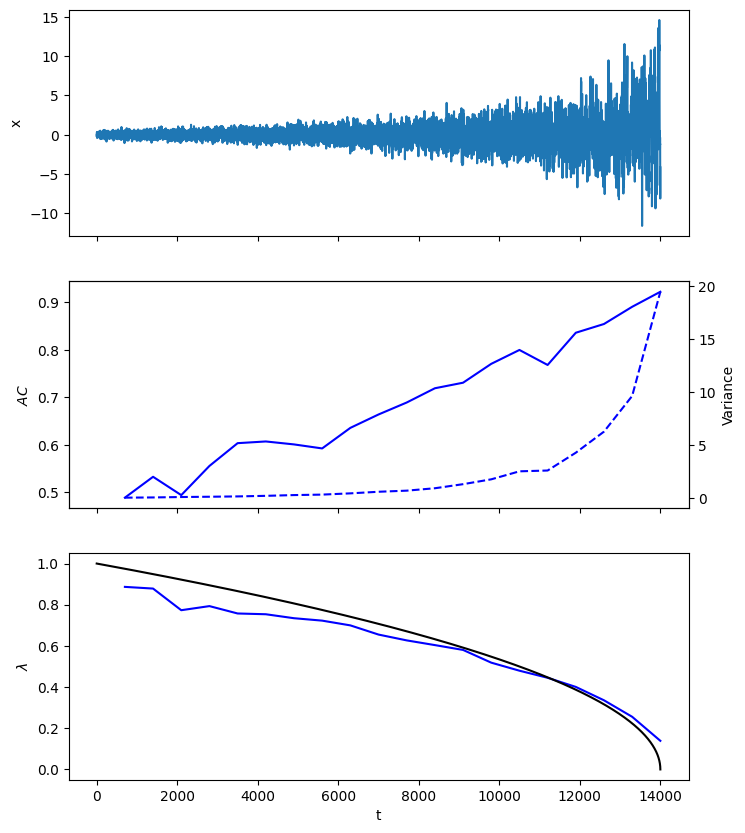
\includegraphics[width=\textwidth]{figures/true_positive.png}
    \end{minipage}
    \hfill
    \begin{minipage}{0.49\textwidth}
        \centering
        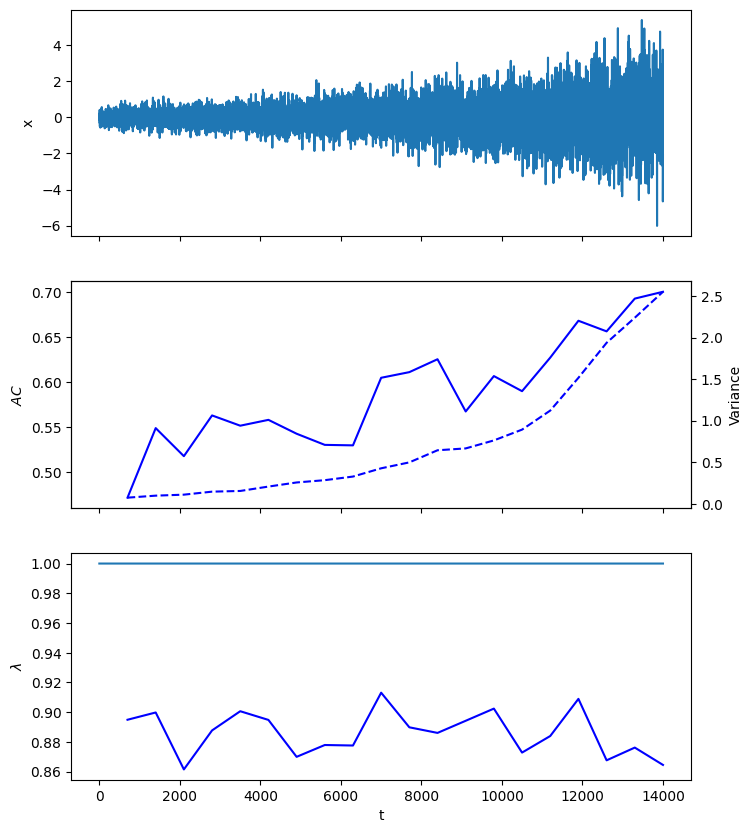
\includegraphics[width=\textwidth]{figures/false_positives.png}
    \end{minipage}
    \begin{minipage}{\textwidth}
    \centering
    \label{false positive}
    modified from \cite{Morr:2024} figure 1, AC: ---, Var: - - -
\end{minipage}

Now we turn to a false negative example. For the simulation of both time series we choose: $(\kappa_{0},\kappa_{T},\theta_{0},\theta_{T}) = (3.2,2.3,1,3.7)$. In this case we have for decreasing $\lambda$ a decline in the variance beside the increase close to T and an increase in AC(1). Hence the variance gives a false negative signal. For fix $\lambda(t) \equiv \lambda_{0}$ both indicators a decreasing. This is again matched by the results from the simulation as seen in \ref{false negative}. The ROSA method again matches $\lambda(t)$ well and doesn't show false signals.


\begin{minipage}{0.49\textwidth}
        \centering
        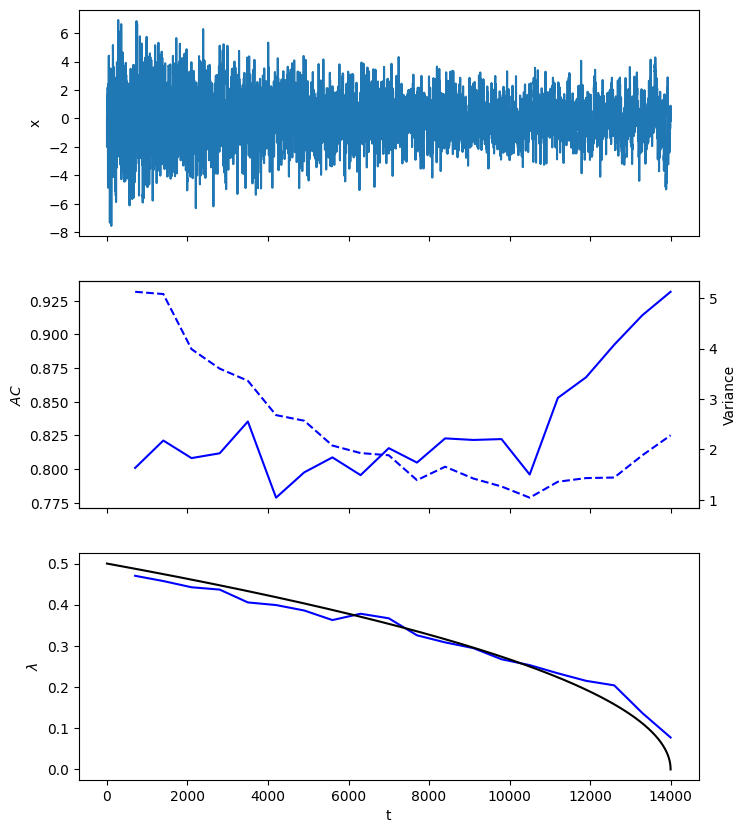
\includegraphics[width=\textwidth]{figures/false_negative_var.png}
    \end{minipage}
    \hfill
    \begin{minipage}{0.49\textwidth}
        \centering
        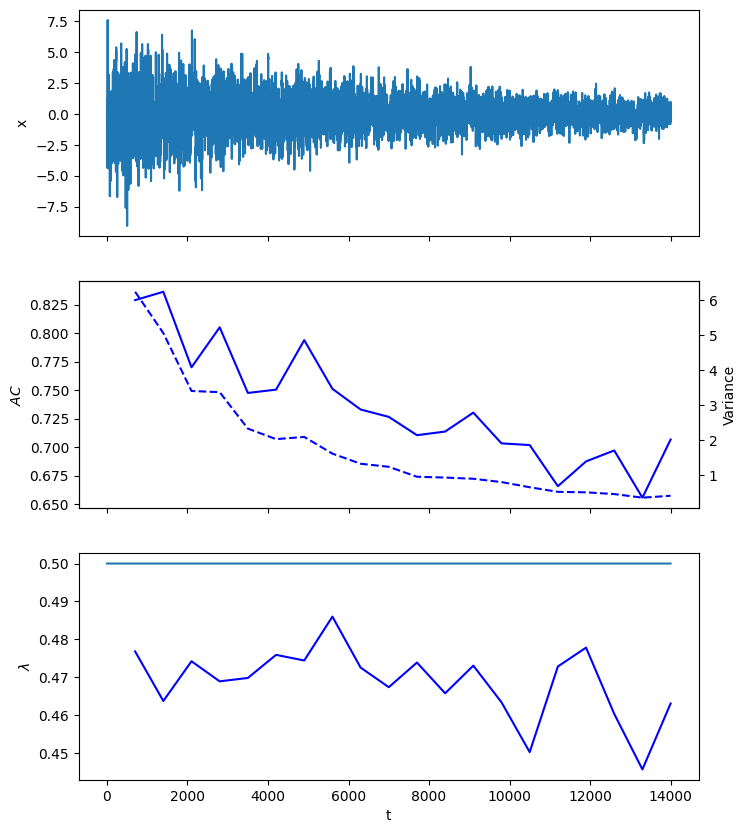
\includegraphics[width=\textwidth]{figures/true_negative.png}
    \end{minipage}
    \begin{minipage}{\textwidth}
    \centering
    \label{false negative}
    modified from \cite{Morr:2024} figure 3, AC: ---, Var: - - -
\end{minipage}

These were however only two examples. We want to provide more evidence for the robustness of the ROSA method, by comparing it to the old indicators on a wider ranch of parameter settings. This will be done in the next chapter.
    


\chapter{Benchmark of traditional EWS with ROSA}

We showed the risk of false signals with the traditional EWS under changing parameters.
The ROSA method showed no wrong signals.
In this chapter we want to carry out a more thorough comparison in terms of false positives vs. true positive of the traditional EWS versus the ROSA method. We do this by plotting the ROC curve and computing the AUC values. First we will do this for 100\% of observed CSD and then for 60\%.

For the comparison we remind us of the test setting: 

\begin{subequations}
    \begin{align*}
        dX_{t} &= -\lambda(t) X_{t}dt + \kappa(t) U_{t}dt, X_{0} = 0 \\
        dU_{t} &= -\theta(t) U_{t}dt + dW_{t}, U_{0} = 0
    \end{align*}
\end{subequations}

Where $\lambda$ either decreases: 
    \[
    \lambda(t) := \lambda_{0}\sqrt{1-t/T}
    \]

Or stays fixed: 
    \[
    \lambda(t)\equiv\lambda_{0}
    \]

We want a reliable indicator, meaning one that leads to as little as possible false positives and as many as possible true positives. All indicators $AC(1),Var,ROSA$ should show an increase for CSD. Hence we have to quantify what we define as a positve signal and what not. To do this we use the Kendall rank correlation coefficient (or Kendall's $\tau$ coefficient) as defined in ~ \ref{def:Kendall tau} and choose a threshold above which we count something as a positive signal. 


The procedure to benchmark our indicators quantitatively is the following:
T = 14000, window length = 700 hence number of disjoint windows = 20, steps per unit time = 10, we choose n = 1000 parameters $(\lambda_{0},\kappa_{0},\kappa_{T},\theta_{0},\theta_{T})$ where $\lambda_{0} \sim \text{Unif}(0.3,0.5)$ and $\kappa_{0},\kappa_{T},\theta_{0},\theta_{T} \sim \text{Unif}(0.5,4)$. For each parameter setting we generate one path where $\lambda(t)$ is decreasing and one where it is not. We do this using the Euler Method. Then we compute the indicators Variance, $AC(1)$ and ROSA for both time series. Afterrwards we calculate the Kendall's $\tau$ value for the indicator series from the three EWS for decreasing and fixed evolution of $\lambda(t)$. We create an array of 1001 threshold values equally spaced between -1 and 1. We compute the true positive rate for all indicators taking the mean of the corresponding Kendall's $\tau$ values of the 1000 settings with a decreasing $\lambda(t)$ that are greater than the threshold. To get the false positive rate, we do the same, now only with the corresponding Kendall's $\tau$ values of the settings with a fixed $\lambda(t)$. Repeat this for all 1001 threshold values. We get the ROC curves by plotting the true positive rates against the false positive rates for the three indicators.
The AUC value is defined as the area under the ROC curve. To compute (approximate: since not actually rectangels, we approximate from above) the AUC values we take the vector of the true positve rates  $tp_{i}, i \in \{Variance,AC(1),ROSA\}$ and the corresponding vector of the false positive rates $fp_{i}, i \in \{Variance,AC(1),ROSA\}$: $fp_{x}^{i} = [0,fp_{i}[1:]-fp_{i}[:-1], i \in \{Variance,AC(1),ROSA\}$ and then $auc_{i} = round(<fp_{x}^{i},tp_{i}>,2), i \in \{Variance,AC(1),ROSA\}$


For a high threshold there is a high proportion of false negative signals for a decreasing $\lambda(t)$. When lowering the threshold for Kendall's $\tau$ from 1 to -1 we would like to have a fast increase in the true positive rate and a slow increase in the false positive rate. Hence a higher AUC value is better. We see that the ROSA method drastically outperforms the two traditional indicators. The $AC(1)$ method is better in detecting CSD then the variance.  
In the ROC curve plot we don't see the spacing of the treshold values. To gain the complete picture we allow for the whole range of Kendall's $\tau$ down to -1 hence counting negative trends as positive signals, which would be odd in practice. We mark the location of the threshold value 0 on the ROC curves. This is the lowest threshold for a reasonable indication of a true positive signal. ? Due to the symmetry of the trends for the null model, the corresponding false positive rate to this point is 50\% ?. In practice we would choose a rather high threshold to increase the significance of positive results and to decrease the false positve rate.

For fold bifurcations a stark decline in the linearized restoring rate shortly before the bifurcation is typicall. However allowing the indicators in our test set up to observe the time series up until the time of tipping is problematic in two ways: it overestimates the usefulness of the indicator since in practice we want an indicator that warns us sufficiently early before tipping; also when approaching the tipping point noise-induced tipping, as described in \ref{fig:1.1} , can't be excluded \cite{Ashwin:2012,Meng:2020}. To assess the capability of the indicators to detect the approaching of a TP early enough, we perform the same analysis, but now only on 60\% of the data. The procedure stays the same, despite now calculating the indicators on only the first 12 = 20 * 0.6 windows. The ROC curve plots for both scenarios (100\% and 60\% of observed Data) are plotted in figure \ref{Figure 9.1}


\begin{figure}[h!]
    \centering
    \begin{minipage}[t]{0.45\textwidth}
        \centering
        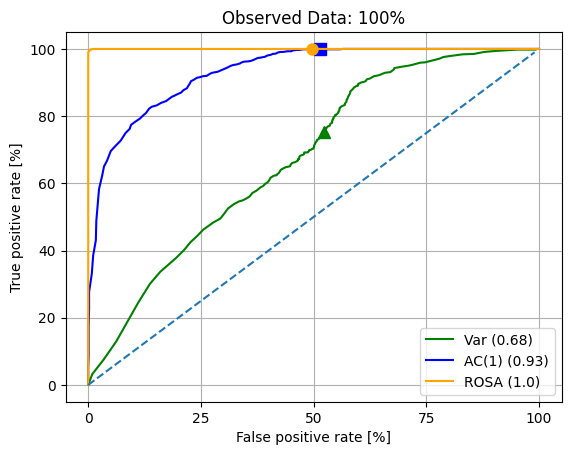
\includegraphics[width=\textwidth]{bachelor-thesis/figures/ROC_curves_100.png}
    \end{minipage}
    \hfill
    \begin{minipage}[t]{0.45\textwidth}
        \centering
        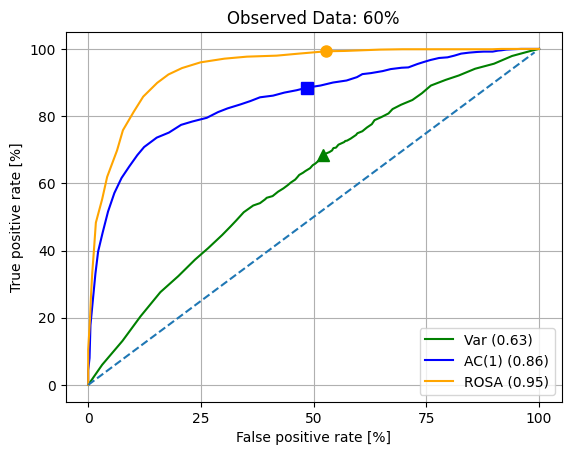
\includegraphics[width=\textwidth]{bachelor-thesis/figures/ROC_curves_60.png}
    \end{minipage}
    \vspace{0.5cm}
    
    % Text below the figures
    \centering
    \begin{minipage}[b]{0.9\textwidth}
        \centering     
        Figure 9.1: modified from \cite{Morr:2024} figure 2. In the left panel the analysis is conducted on the full evolution of $\lambda(t)$. For the AUC values, view the legend. The ROSA method shows perfect differentiation between false positives and true positives. The $AC(1)$ indicator is also significantly better then the variance. The location, where Kendall's $\tau$ is 0, is denoted by the symbols. In the right panel only 60\% of the data was observed. All indicators performed worse as expected, because the sharp decline of the restoring rate is not present in the data and hence the signs of CSD are more subtle. Again the ROSA method outperformed the traditional EWS with the $AC(1)$ being better than the variance.
    \end{minipage}
    \label{fig:figure 9.1}
\end{figure}

in \cite{Morr:2024} Morr proposed three additional indicators $\phi,\lambda^{(ACS)},\lambda^{(PSD)}$. In the case of 100\% observed data the AUC valuess were $\phi [0.99], \lambda^{(ACS)} [1.0], \lambda^{(PSD)} [1.0]$ and in the case of 60\% of observed data it was  $\phi [0.85], \lambda^{(ACS)} [0.94], \lambda^{(PSD)} [0.94]$. (explain these indicators shortly). We see that the ROSA indicator was at least as good as all of these in both cases.
The worse performance of the variance and $AC(1)$ in the case of 60\% observed data is due to the fact, that changes in $\theta$ and $\kappa$ are now often relatively larger than the change in $\lambda(t)$, since the part of the sharp decline is missing now. As we have seen in the previous chapter the changes in $\theta$ and $\kappa$ can hide the true evolution of $\lambda(t)$. The ROSA method performs worse because for cases of true CSD the Kendall $\tau$ value is smaller when only observing 60\% of the data, since the sharp decline is not present. Hence the method detects fewer cases of true positives for a fixed threshold.

We want to further illustrate the dependence of  quality of the indicators on the fraction of observed CSD and the time series length. For the dependence on percentage of observed data we fix the time series length at T = 14000 and let the fractions vary in [0.2,0.4,0.6,0.8,1]. To analyse the dependence on the length of the time series, we fix the fraction of observed data at 60\% and let the time length vary in the range [5000,10000,15000,20000,25000,30000]. We see that the quality of the traditional EWS methods mainly depends on the fraction of observed data, while the length of the time series doesn't play much of a role. Contrary for the ROSA method the power of the method increases both with a higher fraction of observed data as well as with a longer time series. Again the newly proposed EWS is better than the old ones in all cases. 


\begin{figure}[h!]
    \centering
    \begin{minipage}[t]{0.45\textwidth}
        \centering
        \includegraphics[width=\textwidth]{bachelor-thesis/figures/fixed_length_vary_frac_500.png}
    \end{minipage}
    \hfill
    \begin{minipage}[t]{0.45\textwidth}
        \centering
        \includegraphics[width=\textwidth]{bachelor-thesis/figures/fixed_frac_vary_length_500.png}
    \end{minipage}
    \vspace{0.5cm}
    
    % Text below the figures
    \centering
    \begin{minipage}[b]{0.9\textwidth}
        \centering     
        Figure 9.2: 
    \end{minipage}
    \label{fig:figure 9.2}
\end{figure}


\chapter{ROSA applied to the Snowball earth modell}

In this section we would like to apply the ROSA method to a climate modell, where tipping occurs due to a fold-bifurcation: the Snowball Earth model, which is a simple Energy Balance Model (EBM). First we shortly discuss the theory behind these simple models, taken from \cite{Kaper:2013}. The key quantity of Earth's climate system is temperature. In an EBM the state of Earth's climate is summarized in the variable temperature averaged over the entire globe. The simplest EBM doesn't cover any spatial dimensions and is thus sometimes referred to as zero-dimensional EBM. It is governed by an ODE. To derive this ODE we have to consider the energy budget of the Earth.

Almost all the energy for Earth's climate system comes from the sun in the form of electromagnetic radiation. A part of this is absorped by the solar photosphere (the outer shell of a star). Treating the sun as a black body at 5780K temperature is a good approximation for the solar energy spectrum.

The flux of solar radiation through a unit area of a sphere at a distance of one astronomical unit away from the sun is called the solar constant measures and is measured as $1,368Wm^{-2}$. Due to the sunspot cycle it is not exactly constant but varies around $0.1\%$

The incident solar radiation (insolation) is more precise. It refers to the energy per unit area at a particular point in time and space. In contrast to the solar constant the insolation varies significantly  with time of day, season, latitude etc. To keep our model simple we stay with the solar constant.

When we neglect the differences among continents and oceans, in the composition of the atmosphere, topography and other local features, we can characterise the state of the entire earth system by the single variable global mean surface temperature T. We want to know how T evolves over time. Though there are many complicated processes involved in determining T, we know that T will increase if the energy from the sun reaching Earth's surface exceeds the amount of energy emitted by Earth and vice versa.
The heat capacity of a system is the amount of energy needed to raise the temperature by one degree Celsius/Kelvin and is measured in watt years per square meter [$W yr m^{-2}$]. For simplicity we don't differentiate the heat capacity for different mediums and just consider it as the constant average value $C$ for the whole globe. If $A$ is the surface area of the earth and we have $T(t+\Delta t) = T(t) + \Delta T$, than we need $AC\Delta T$ energy to reach this new temperature.  Let $E_{in}$  ($E_{out}$) be the mean level of energy reaching (leaving) one square meter of the Earth's surface per unit time. Then we get: 
\begin{equation}
AC\Delta T = A(E_{in} - E_{out})\Delta t
\end{equation}
After canceling A, dividing by $\Delta t$ and letting it go to zero we get the following 0-dimensional EBM: 
\begin{equation}
    C\frac{dT}{dt} = E_{in} - E_{out}
\end{equation}
In an equilibrium we have $E_{in} = E_{out}$. Next we want to find simple expressions for $E_{in}$ and $E_{out}$.

We start with a basic model.
Be $R$ the radius of the Earth and $S_{0}$ the solar constant. If we would look at the Earth from the sun it would appear as a flat disc with surface area $\pi R^2$. The Earth thus receives $\pi R^2 S_{0}$ solar energy per unit time. Only a fraction $1-\alpha$ of this reaches the surface, where $\alpha \in (0,1)$ is the so called \textit{albedo} - the fraction reflected back to space. Locally the albedo differs drastically. Ice sheets for example reflect much more back than a desert does. For now we will again average the albedo over the entire globe. The energy $(1-\alpha)\pi R^2S_{0}$ is uniformly distributed over the Earth's surface area which is $4\pi R^2$. Hence the amount of Energy per square meter per unit time is $\frac{(1-\alpha)\pi R^2S_{0}}{(4\pi R^2)} = \frac{1}{4}(1-\alpha)S_{0}$. With $Q:=\frac{1}{4}S_{0}$ we get: 
\begin{equation}
    E_{in} = (1-\alpha)Q
\end{equation}
Now we consider $E_{out}$. The Earth also emits electromagnetic radiation, but mostly very long waves (infrared regime). We approximate the Earth as a black body with surface temperature $T$.Then according to the Stefan-Boltzmann law, the earth radiates 
\begin{equation}
    E_{out}(T) = \sigma T^4
\end{equation}
per unit area and per unit time, where $\sigma = 5.67 \cdot 10^{-8}Wm^{-2}K^{-4}$ is the Stefan's constant. In total we get: 
\begin{equation}
    C\frac{dT}{dt} = (1-\alpha)Q - \sigma T^4
\end{equation}
Setting the right hand side to zero we get the energy balance equation: 
\begin{equation}
    (1-\alpha)Q = \sigma T^4
\end{equation}
Solving for T: 
\begin{equation}
    T^* = (\frac{(1-\alpha)Q}{\sigma})^\frac{1}{4}
\end{equation}
With $Q = \frac{1}{4}S_{0}= 342 Wm^{-2}$ and $\alpha = 0.3$, which is a common value for Earth's albedo, we get an equilibrium temperature of $T^* = 254.8K$. This is much colder than our real surface temperature of $287.7K$. In the next paragraph. we will include the greenhouse effect into our model, which can explain a large part of the difference.
\\ 
Greenhouse gases like carbon dioxide ($CO_{2}$), methane, water vapor and aerosols (dust particles, water droplets, etc.) increase the opacity of the atmosphere in the infrared regime (wavelengths greater than $0.7 \mu m$). Due to the very different emitting temperatures of Earth and Sun their emitting regimes barely intersect (Fig 2.4). While the sun emits only waves with length below $4 \mu m$ the earth emits only waves with lengths greater than $4 \mu m$. Hence the greenhouse effect decreases $E_{out}$ and has no impact on $E_{in}$. Therefore the global mean temperature increases. We incorporate this effect on $E_{out}$ by multiplying it with a factor $\epsilon \in (0,1)$. The modified energy balance equation: 
\begin{equation}
    (1-\alpha)Q = \epsilon \sigma T^4
\end{equation}
has the solution: 
\begin{equation}
    T^* = (\frac{(1-\alpha)Q}{\epsilon\sigma})^\frac{1}{4}
\end{equation}
We can get T* = 287.7K when we artificially choose $\epsilon = 0.62$, keeping $\alpha = 0.3$ and $S_{0} = 1,368 Wm^{-2}$. 
Now we want to improve our model further. 

A temperature independent albedo does not account for the fact that snow and ice reflect sunlight much better than open water. We will include this observation into our simple model from (5) by setting 
\begin{equation}
    \alpha (T) = 0.5 - 0.2 \cdot tanh(\frac{T - 265}{10})
\end{equation}
This gives us: 
\[
\alpha(T) =
\begin{cases}
0.7 & \text{if } T < 250K \\
0.3 & \text{if } T > 280K
\end{cases}
\]
This makes sure that a larger proportion of energy is reflected back to space, when the temperature is low enough for the earth to be covered by ice and snow.
The energy balance equation with a temperature dependent $E_{in}$: 
\[
 C\frac{dT}{dt} = (1-\alpha(T)Q - \epsilon\sigma T^4
\]
Below we plot $(1-\alpha(T))Q$ and $\epsilon\sigma T^4$ against $T$. We see that there are three equilibria at $T_{1}^* = 288K$, $T_{2}^* = 265K$ and $T_{3}^* = 233K$, where $T_{1}^*$ and $T_{3}^*$ are stable and $T_{2}^*$ is unstable. Our current climate corresponds to $T_{1}^*$. In the \textit{Snowball Earth} scenario $T_{3}^*$ the earth would be entirely covered by snow and ice. 

\begin{figure}
    \centering
    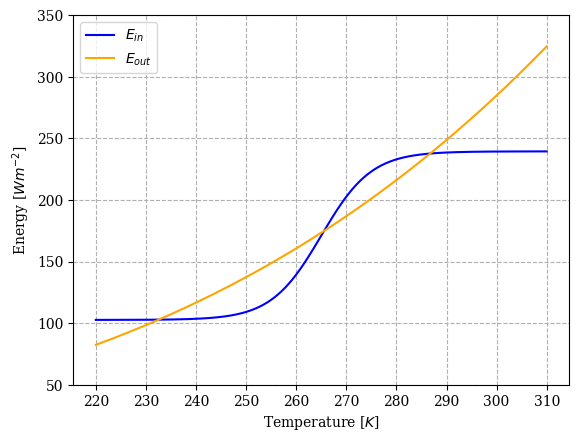
\includegraphics[width=0.7\textwidth]{bachelor-thesis/figures/se_multiple_equilibria.png}
    \caption{modified from \cite{Kaper:2013} figure 2.5}
    \label{fig:enter-label}
\end{figure}

We have to keep in mind that the time scale of an EBM covers millions of years. Hence all recent ice ages and the most severe periods of glaciation of the last million years correspond to the state $T_{1}^*$. The question arises though, whether the planet has visited the state $T_{3}^*$ in the past. There is some geological evidence suggesting that the Earth was completely frozen during the Cryogenian (720-635 Myrs BP) and Huronian (2400 - 2100 Myrs BP) age (Lecture 2 Boers) (Engler: 4 times during 750-580 neoproterozoic age). How could the earth escape this state of complete glaciation? There was still some CO2 released into the atmosphere e.g. from volcanic erruptions, but no biomass existed that could take this up. This lead to a large accumulation of CO2 and consequently an increase in the greenhouse effect. In our simple model this corresponds to a decrease of $\epsilon$ and the orange curve. At some point the stable equilibrium $T_{3}^*$ would vanish and the climate system would suddenly transition to a much warmer stable equilibrium. Paleoclimate reccords exist that provide evidence for such rapid change at the end of glaciation periods (Cambrian explosion). Other questions that come to mind are: why wasn't there a snowball earth period during the last 500 million years and could there be another one in the future? We know that the continents were closer to the equator during the proterozoic age and that rock-erosion is a main actor in the removal of CO2. This lead to a low level of CO2 and greenhouse gas effect, while the polor caps could expand during ice ages. With todays distribution of the continents being closer to the poles the rock erosion would end earlier during an ice age, leading to an earlier regulating effect due to the greenhouse gas effect. During the cold war there was the fear that an outbreak of a nuclear war could cause the earth to freeze. 

Now we want to understand how the equilibrium states develope when we change the solar constant $S_{0}$. To do this we plot the bifurcation diagram below. We have a fold bifurcation model with bifurcation points at $Q_{-}$ and $Q_{+}$. Here $q := Q/Q_{0}$ is the bifurcation parameter, where $Q_{0} = 342 Wm^{-2}$. When we let $q$ cross $Q_{-}$ from above, then $T_{1}^*$ and $T_{2}^*$ merge and disappear, leading to the snowball earth state $T_{3}^*$ (lower branch). If we cross $Q_{+}$ from below, then we only have the state $T_{1}^*$ (upper branch) free of ice. We also notice that there is hysteresis build into the system. 

In the next step we want to apply the traditional EWS and ROSA method to our simple EBM.
The simulation works the same as for the abstract setting from the last chapter only now with a different function used for the SDE. We let our time series start in the lower branch and linearly increase $q$ until it tips over into the upper branch. In the upper panel of fig \ref{fig:ROSA test} we see the full picture, where $q$ ranges from 0.7 to 1.4. We observe that the rate $-\lambda(t)$ first increases before going to zero. In the previous sections we always had the case that we computed our EWS only on the already decreasing part of $-\lambda$. As we see here this doesn't have to be the case in general. To better compare our methods we simulate the time series again in the more crucial region of $q \in [1.1,1.3]$ as illustrated in the lower row of \ref{fig:ROSA test}. In the left panel the system is driven by white noise and all methods show an increase as expected (kendalltaus: $AC(1)$ (0.3142857142857143), Variance (0.40952380952380957), ROSA (0.8857142857142857)) whereas in the right panel we provoke a false negative for the traditional EWS by linearly decreasing $\kappa$ (from 3.2 to 2.3) and linearly increasing $\theta$ (from 1 to 3.7). The ROSA method also works in the red noise case. (ROSA more monotonic: earlier detectable).

\begin{figure}[t]
    \centering
    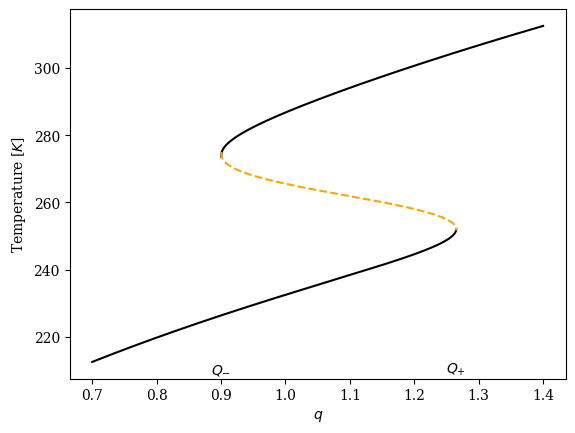
\includegraphics[width=0.6\textwidth]{bachelor-thesis/figures/se_bif_plot.png}
    \caption{modified from \cite{Kaper:2013} figure 2.6}
    \label{fig:se_bif}
\end{figure}



\begin{figure}[b]
    \centering
    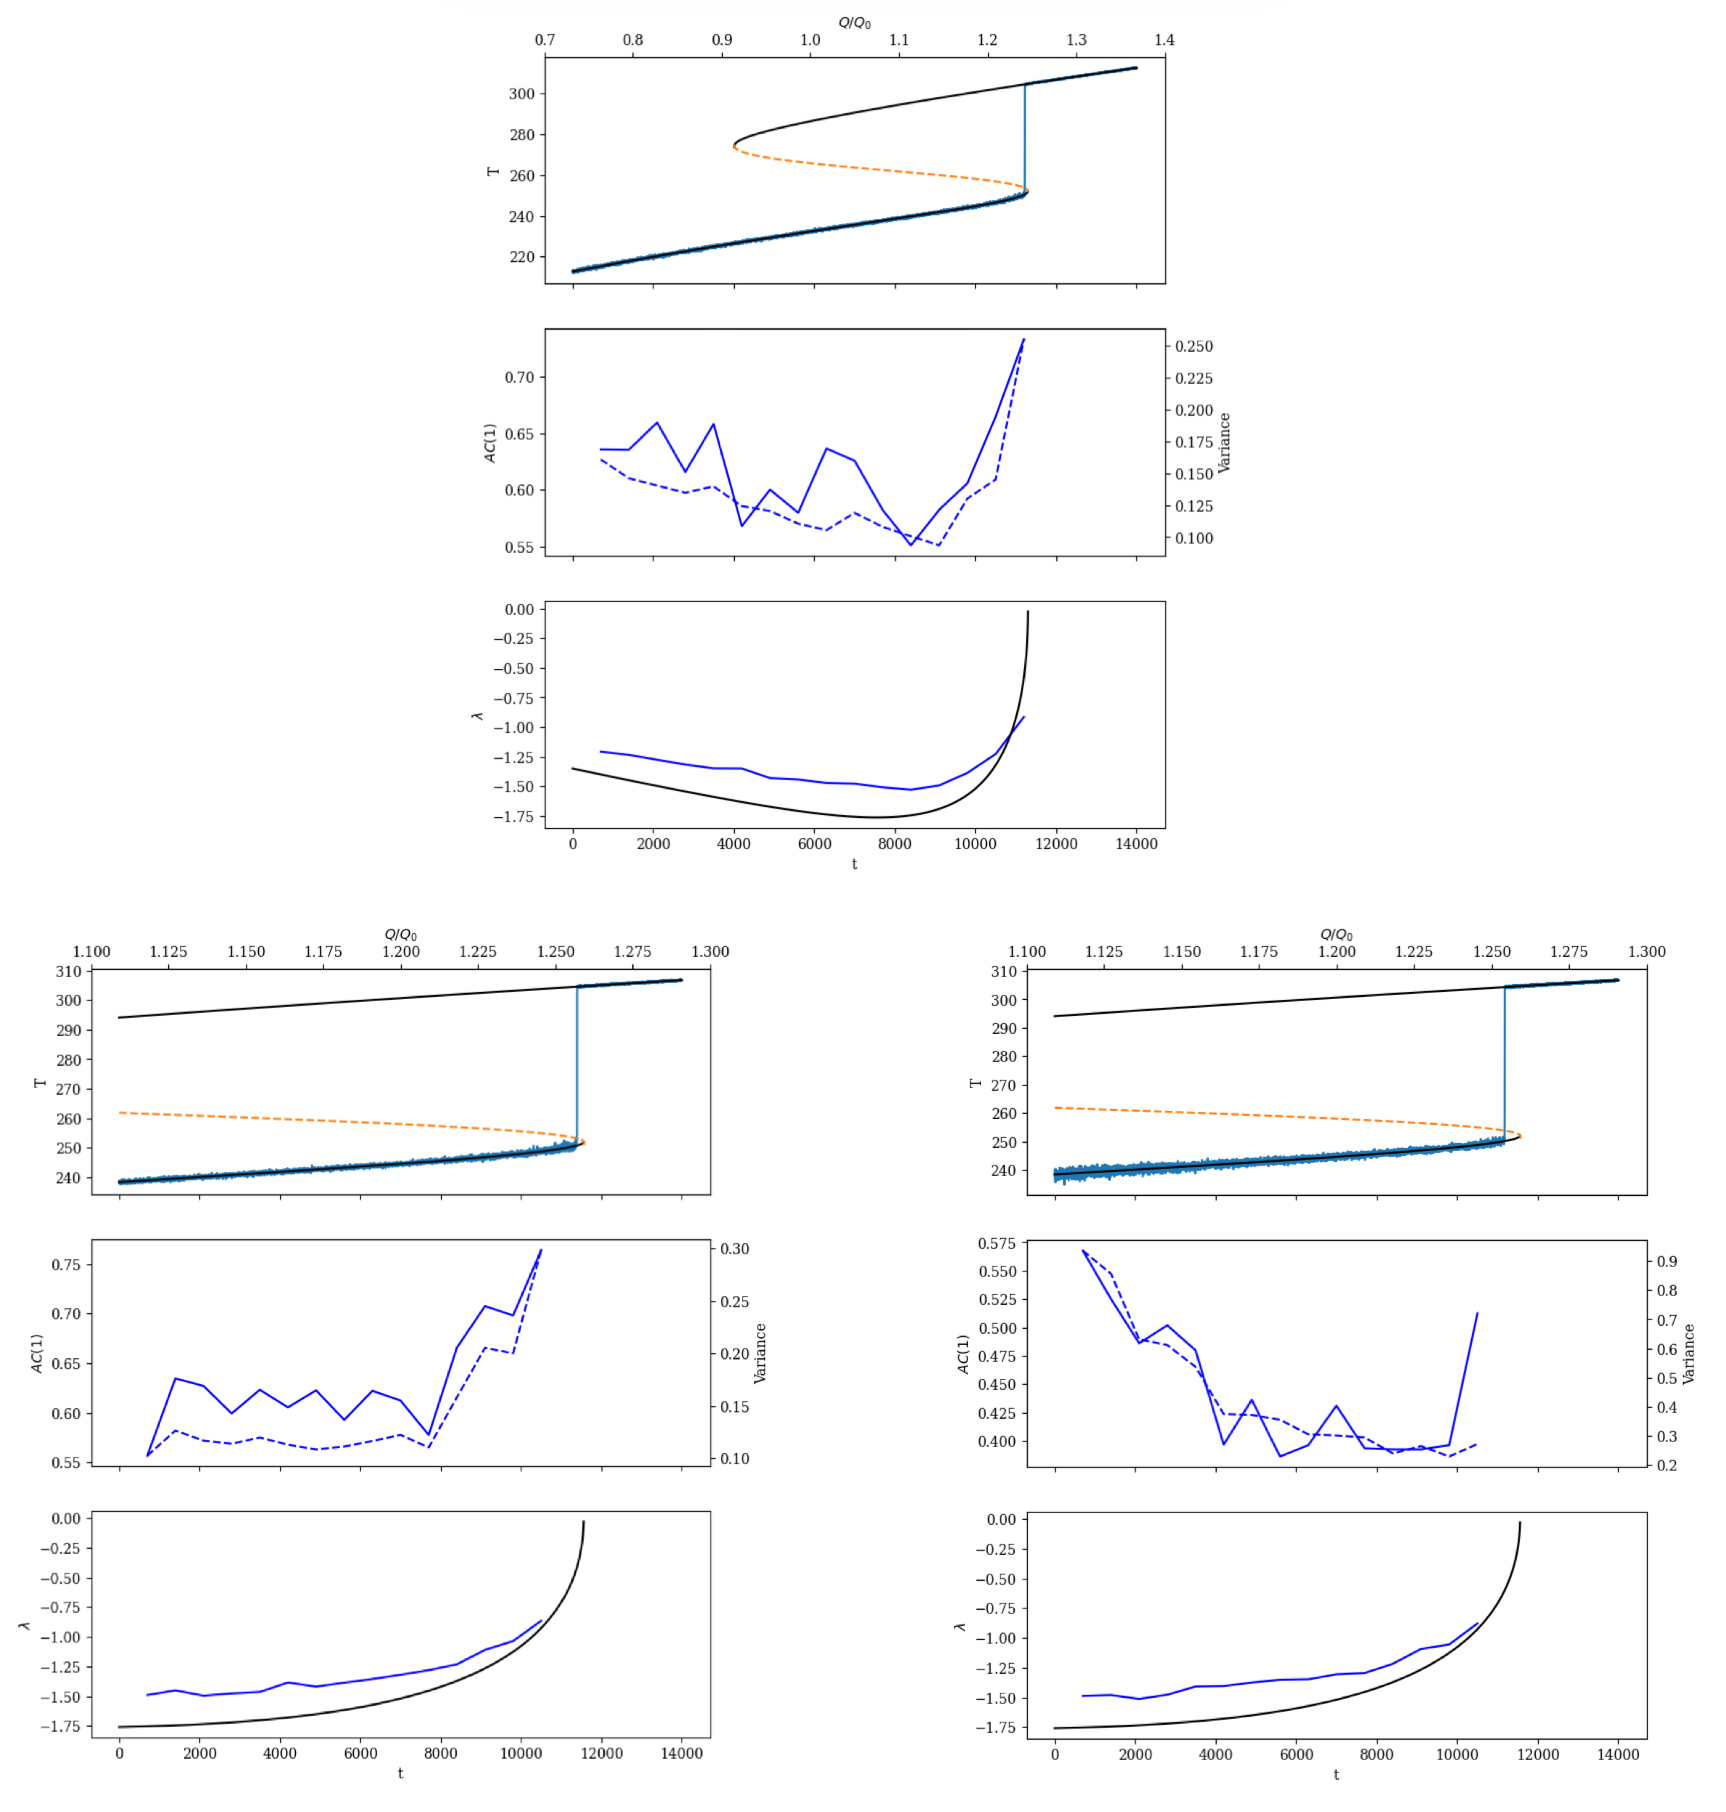
\includegraphics[width=0.9\textwidth]{bachelor-thesis/figures/ROSA_test_se.jpg}
    \caption{ROSA test}
    \label{fig:ROSA test}
\end{figure}



\appendix
\chapter{Appendix}
\section{Supporting Data}
\section{Some Code Listings}

\backmatter{}
\listoffigures% may be removed
\listoftables% may be removed

\nocite{Alspach:2008,GaleShapley:1962} % further literature that has not been explicitly referenced in the text
\printbibliography{} % print bibliography

\end{document}

%%% Local Variables:
%%% mode: latex
%%% TeX-engine: default
%%% TeX-command-extra-options: "-shell-escape"
%%% ispell-local-dictionary: "american"
%%% eval: (setenv "TEXINPUTS" ".//:")
%%% TeX-master: t
%%% End:
